%====================================================================================================
% Controle PID
%====================================================================================================
% Plano de Trabalho
%----------------------------------------------------------------------------------------------------
% Autor			: Kelvim Rodrigues de Oliveira	
% Orientador		: Gedson Faria
% Instituição 		: UFMS - Universidade Federal do Mato Grosso do Sul
% Unidade		: CPCX - Campus de Coxim
%----------------------------------------------------------------------------------------------------
% Arquivo		: plano_trab_kelvim.tex
% Data de criação	: 13 de Maio de 2017
%====================================================================================================

\documentclass[a4paper,12pt,portuguese]{ufms-cpcx}


\usepackage{amsmath,amssymb,latexsym}
\usepackage{float}
\usepackage{xcolor}
\usepackage{listings}
\usepackage[utf8]{inputenc}
\usepackage[top=30mm,bottom=25mm,left=25mm,right=20mm]{geometry}
\usepackage{pdfpages}
\usepackage [onehalfspacing]{setspace} 
\usepackage{indentfirst}
%\usepackage{caption}
\usepackage[font=small]{caption}
\usepackage{subcaption}
\usepackage{multicol}
\usepackage{booktabs}	% http://ctan.org/pkg/booktabs
\usepackage{array}	% http://ctan.org/pkg/array


\newcolumntype{M}{>{\centering\arraybackslash}m{\dimexpr.25\linewidth-2\tabcolsep}}

\lstset{
	language=C++,
	basicstyle=\ttfamily\small, 
	keywordstyle=\color{blue}, 
	stringstyle=\color{verde}, 
	commentstyle=\color{red}, 
	extendedchars=true, 
	showspaces=false, 
	showstringspaces=false, 
	numbers=left,
	numberstyle=\tiny,
	breaklines=true, 
	backgroundcolor=\color{green!10},
	breakautoindent=true, 
	captionpos=b,
	xleftmargin=0pt,
}

\begin{document}
\definecolor{verde}{rgb}{0,0.5,0}
\thispagestyle{empty}



\titulo{ Monografia apresentada\vskip 1.5cm 
	para obtenção de controle equilibrado de velocidade.}\vskip 0.5cm
\autor{Kelvim Rodrigues de Oliveira}

\orientacao{Prof. Dr. Gedson Faria}
%\docarea{Bacharelado em Sistemas de Informação}
\textofree{\large Bacharelado em Sistemas de Informação}

\vfill \centerline{
\includegraphics[scale=0.15]{figuras/ufms-logo.jpg}}

\vskip 0.5cm
\begin{center}
	Universidade Federal de Mato Grosso do Sul\\ 
	Campus de Coxim\\ \vskip 1.0cm
	13 de Maio de 2017
\end{center}

\chapter*{}

\begin{center}
	
	\begin{minipage}[t]{10cm}
		\begin{center}
			\vspace{-2cm}
			{{\Large Controle equilibrado de velocidade.}}  
		\end{center}
	\end{minipage}
	
\end{center}

\vskip 3.0cm \textofree{\large Monografia apresentada para obtenção de controle equilibrado de velocidade.}

\begin{flushright}
	\vspace{12cm}
	Coxim, 13 de Maio de 2017.
\end{flushright}

%\vspace{2cm}



%\tableofcontents

%\printglossaries

%\cleardoublepage
%\phantomsection
%\addcontentsline{toc}{chapter}{Lista de Tabelas}
%\listoftables



\chapter{Introdução}
Bla bla bla
 
 
 \section{Justificativa}  
 Bla bla bla


 \section{Objetivos}
 
 
 \section{Objetivo Geral}  
  
 O objetivo deste trabalho é estudar e implementar controle de velocidade entre os motores esquerdo e direito do robô jogador. 

\section{Objetivos Específicos}

\begin{itemize}
	%lista de itens	
	
	\item Criar uma interface simples e intuitiva para que qualquer pessoa sem alto nível de conhecimento no pacote \textit{Vaucanson-G} possa utilizá-lo.
	
	\item Desenvolver o sistema de transição livre.
	
	\item Desenvolver o sistema de transição dupla.
	
	
\end{itemize}

\section {Organização da Monografia}

\chapter{Revisão da Literatura}

\chapter{Futebol de robôs}
%Este capitulo destina-se alguns conceitos, informações e história do futebol de robôs, suas principais modalidades, dinâmica de jogo e movimentos.
%

\section{Uma breve história sobre futebol de robôs}
Com duas organizações de referencia mundial para o estudo e organização quanto ao futebol de robôs, são elas a FIRA, sigla em inglês para \textit{Federation of International Robot-soccer Association} e a RoboCup associaçães que tem como objetivo promover pesquisas nas áreas de robótica e inteligência artificial, estimulando o interesse dos participantes a resolver problemas. 

A FIRA, fundada no ano de 1995 pelo professor Kim Jong-Hwan, realizou seu primeiro campeonato mundial na Coréia em 1997, dois anos após sua fundação, com o objetivo de levar aos leigos e as gerações jovens o espírito da ciência e tecnologia aplicada à robótica. Desde então, a FIRA vem realizando diversos eventos em vários
países do mundo, incluindo nossa pátria, o que fez com que o futebol de robôs obtivesse reconhecimento mundial. O Brasil, teve a oportunidade de sediar a Copa do Mundo em agosto de 1999, realizada entre os dias 4 a 8, na cidade Campinas no estado de São Paulo.

A RoboCup foi criada no Japão por meio da iniciativa de um grupo de pesquisadores que tinham como objetivo em comum, o jogo de futebol com a finalidade de promover o crescimento da ciência e tecnologia. De forma independente, os professores Minoru Asada da Universidade de Osaka, e a Professora Manuela Veloso junto a seu aluno Peter Stone da Universidade Carnegie Mellon, EUA, estavam também trabalhando em robôs jogadores de futebol.
O primeiro campeonato da Robocup junto a primeira conferência, foram realizados em 1997, onde compareceram mais de 40 equipes e mais de 5.000 espectadores. Infelizmente no Brasil até o momento não foram realizados eventos da Robocup com âmbito mundial.

\section{Modalidade} \label{modalidade}
Assim como o futebol jogado por humanos, o futebol de robôs também tem suas regras de jogo bem definidas. A FIRA Cup é um evento organizado com competições várias categorias, destacam-se as categorias \textit{Micro-Robot Soccer Tournament} (MiroSot) e a \textit{Humanoid Robot Soccer Tournament} (HuroSot), ambas são disputadas sob o olhar de um árbitro humano, já a categoria \textit{Simulated Robot Soccer Tournament} (SimuroSot), que como o próprio nome sugere, trata-se de uma modalidade de simulação, quando não se tem a disposição de os recursos de hardware referentes aos robôs.
 
Este trabalho tem como foco o estudo das velocidades dos motores da categoria \textbf{VSS} do inglês \textit{\textbf{IEEE Very Small Size}} a competição ocorre durante a RoboCup, a versão sul-americana da competição, cuja categoria é voltada para partidas com pequenos robôs que se movimentam através de dois motor, um motor para cada roda, realizando movimentos rápidos, os robôs são controlados remotamente, mas sem intervenção humana, os comandos são enviados a partir de um computador disposto com uma inteligencia artificial e suas estratégias, está inteligencia por sua vez utiliza-se do processamento das imagens de vido das câmeras dispostas em cima do campo. Sendo este o ambiente principal do trabalho.
A partida deve ser jogada por duas equipes, com três robôs cada, um robô pode atuar como goleiro de acordo com as estratégias, já fora de campo o time contem três membros humanos, o ``gerente", o ``técnico" e um ``instrutor" os quais só tem acesso ao palco. Cada equipe possui seu computador o qual é principalmente dedicado ao processamento de visão, identificação e de localização.  
O tamanho dos robôs desta categoria é limitado a 7,5 cm x 7,5 cm x 7,5 cm, altura da antena não deve ser considerada na medição do tamanho de um robô, é utilizado uma bola de golfe de cor laranja afim de facilitar o processo de visão computacional.
Esta categoria conta com duas ligas, a ``\textit{Large league}" (Liga grande) considerado grande pois o seu campo possui as dimensões de 400cm x 280cm e a ``\textit{Middle league}" (Liga média) que tem seu campo menor com as dimensões de 220cm x 180cm.

======== INSERIR IMAGEM DAS DIMENSÕES DO CAMPO =========

\chapter{O robô}
O time de futebol de robôs do campus de Coxim enquadra-se na modalidade VSS confome a seção \ref{modalidade} esta limitado as dimensões de 7,5 cm x 7,5 cm x 7,5 cm. Dotado de um Arduino nano o qual realiza o controle de todo o robô, um bluetooth do modelo \textbf{HC-06} \ref{bthc06} que possui apenas o modo \textit{slave}(apenas recebe conexão, não busca a mesma) cujo função principal é estabelecer a conexão entre o robô e o computador da equipe, um driver para motor de corrente continua do modelo \textbf{TB6612FNG} \ref{TB6612FNG} capais de controlar dois motores, dos quais são utilizados para realizar os movimentos, dois sensores ópticos do modelo \textbf{TCRT1000} \ref{TCRT1000} os quais são utilizados em conjunto com as rodas \ref{roda} então este conjunto trabalha como um encoder, utilizado para determinar a velocidade de rotação das rodas/motor.
\begin{figure}[H]
	\centering
	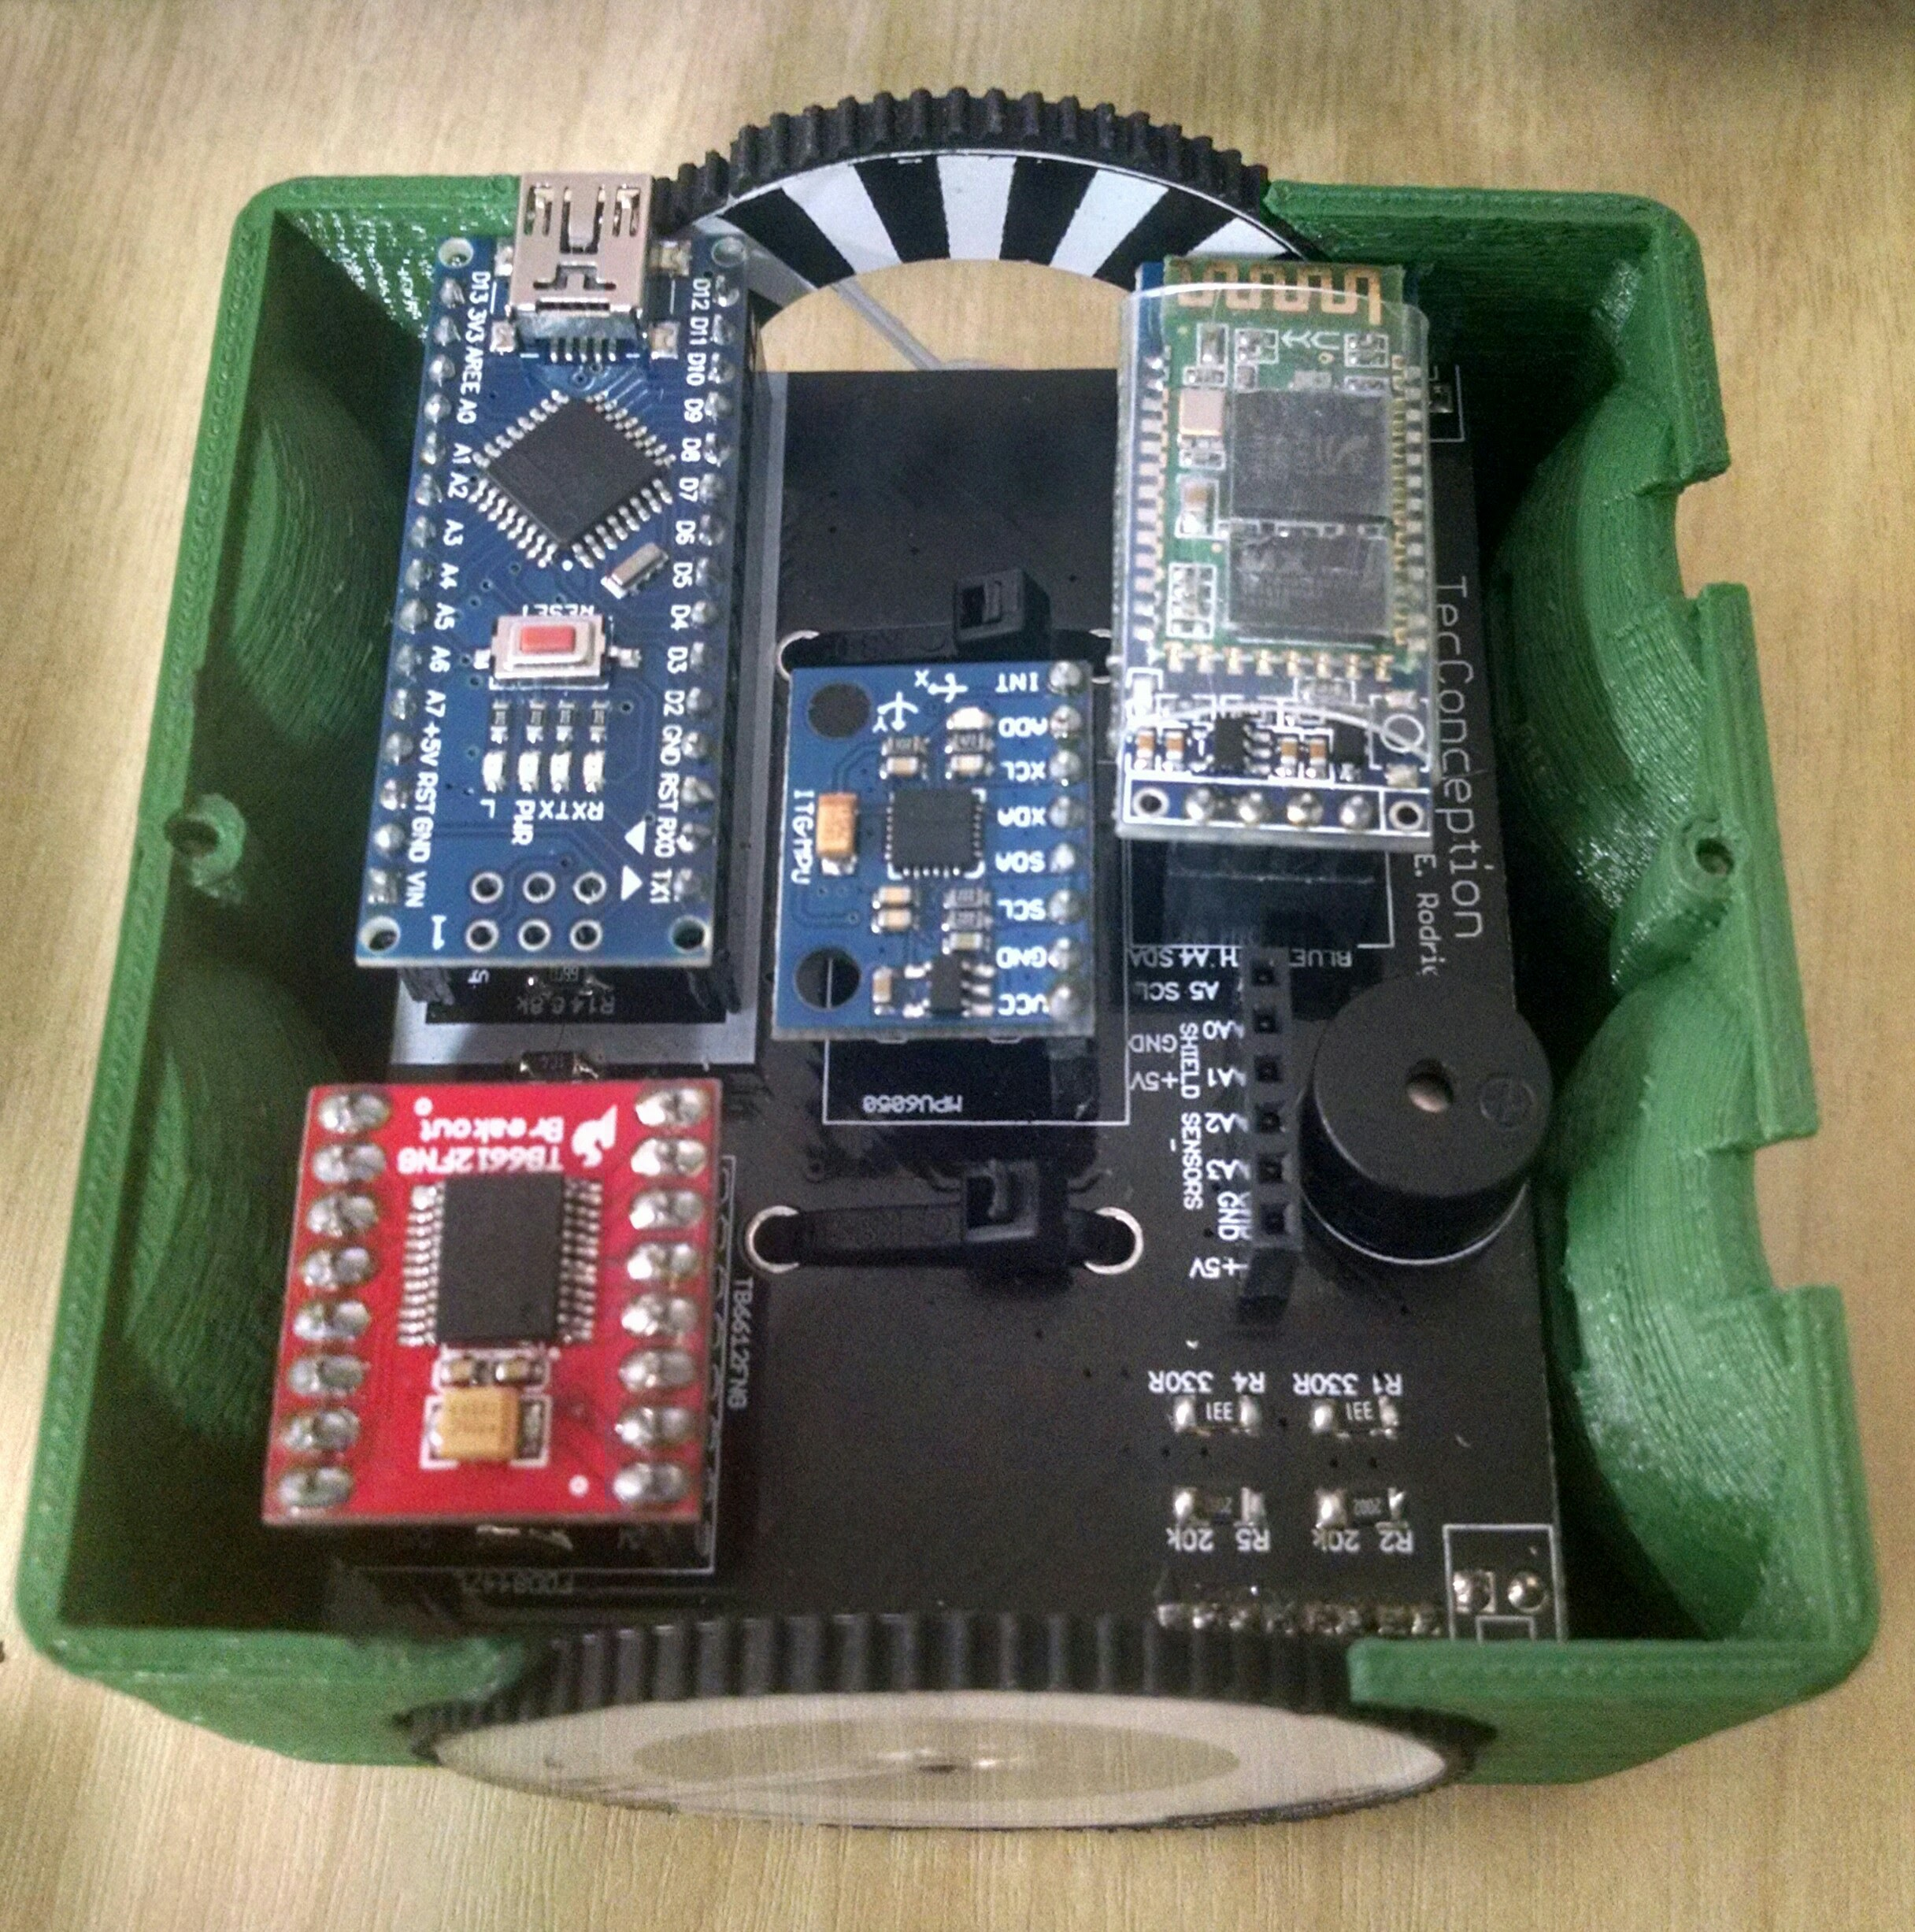
\includegraphics[width=0.5\textwidth]{superiormodu.jpg}
	\caption{Vista superior do robô Modu.}
\end{figure}
\begin{figure}[H]
	\centering
	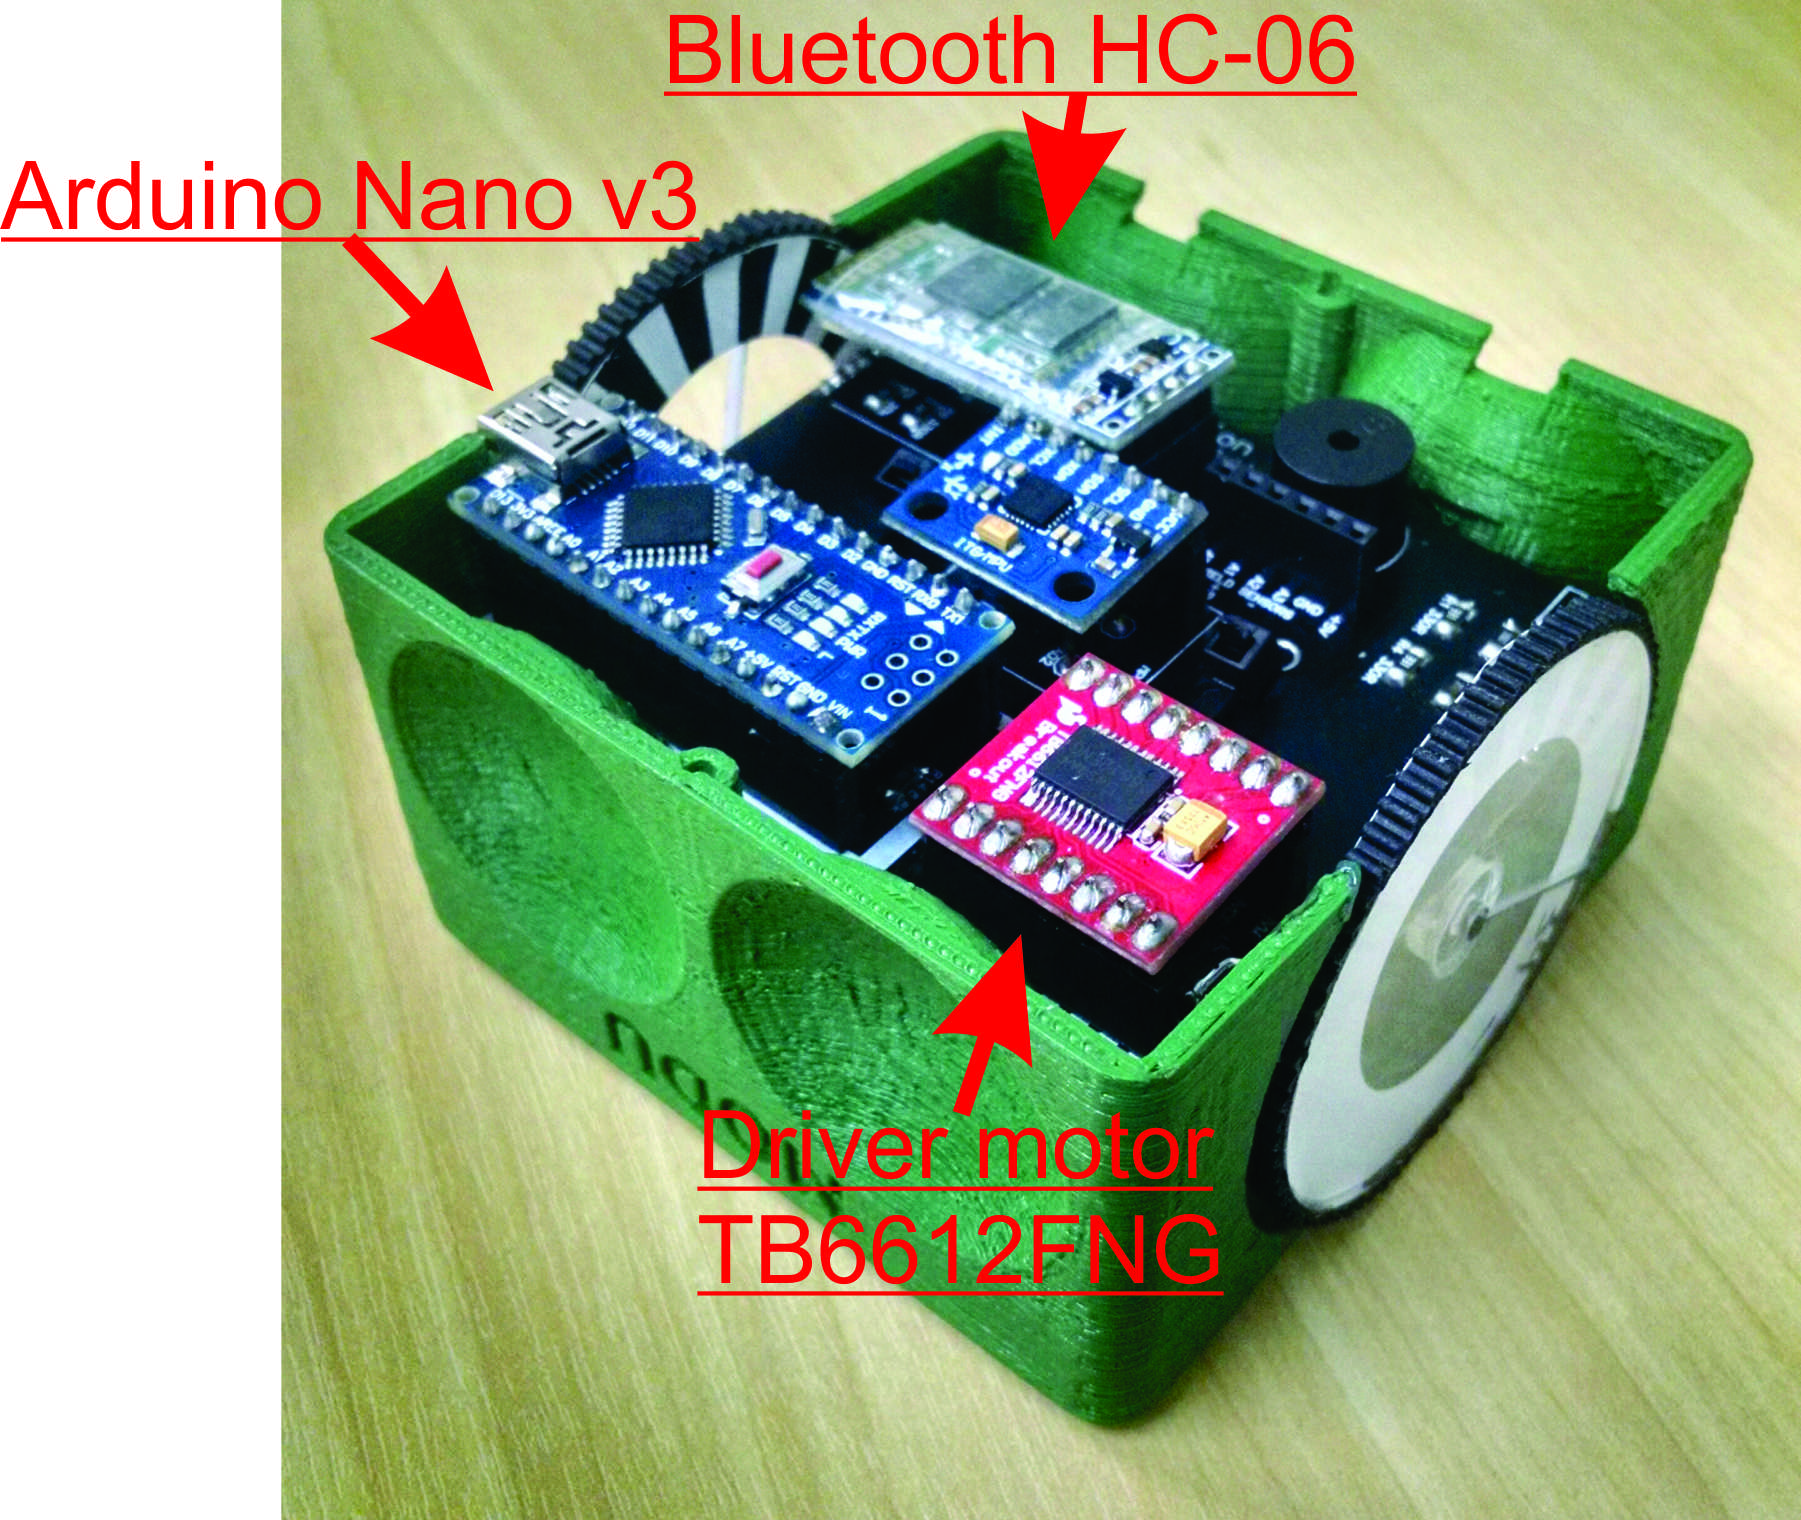
\includegraphics[width=0.5\textwidth]{inferiormodu.jpg}
	\caption{Vista inferior aberto do robô Modu.}
\end{figure}


\section{Arduino}\label{arduinonano}
Todas as versões do Arduino são baseadas em um microprocessador Atmel AVR de 8 bits de arquitetura RISC\cite{arduinoemacao}. O Arduino Nano versão 3.0 utilizado neste projeto, possui um processador ATmega328 provido de uma memória flash de 32 KB no total, sendo 2 KB utilizados pelo \textit{bootloader} deixando disponível 30 KB, com uma velocidade de clock de 16 MHz. Contem uma porta mini-USB integrada que serve para troca de dados e também como fornecimento de energia. O Arduino Nano tem a opção de receber energia também pelo pino 30(VIN) em tensões de 6 a 20 volts e/ou pelo pino 27(5V) uma tensão regulada de 5,5 volts, caso estejam as três fontes de energias conectadas a placa seleciona a de maior tensão para seu funcionamento. Dotado também de uma comunicação serial que possibilita o Arduino se comunicar com um computador ou com outros dispositivos, como o bluetooth neste projeto, o Arduino nano possuem uma porta serial, também chamada UART ou USART, são acessadas pelos pinos digitais 0 (RX) e 1 (TX), assim como uma conexão USB, por isso é necessário um driver serial para utiliza-lo junto ao computador. Sendo assim quando se esta funcionalidade, os pinos 0 e 1 não poderão ser utilizados como entrada ou saída digital.
Na IDE do Arduino existem uma ferramente onde você pode monitorar a comunicação Serial entre a placa do Arduino e o computador.
Componente então de grande utilidade, capacidade, de pequenas dimensões -18 mm x 45 mm- e pesando apenas 7 gramas o tornam ideal para um robô jogador de futebol. 
\begin{figure}[H]
	\centering
	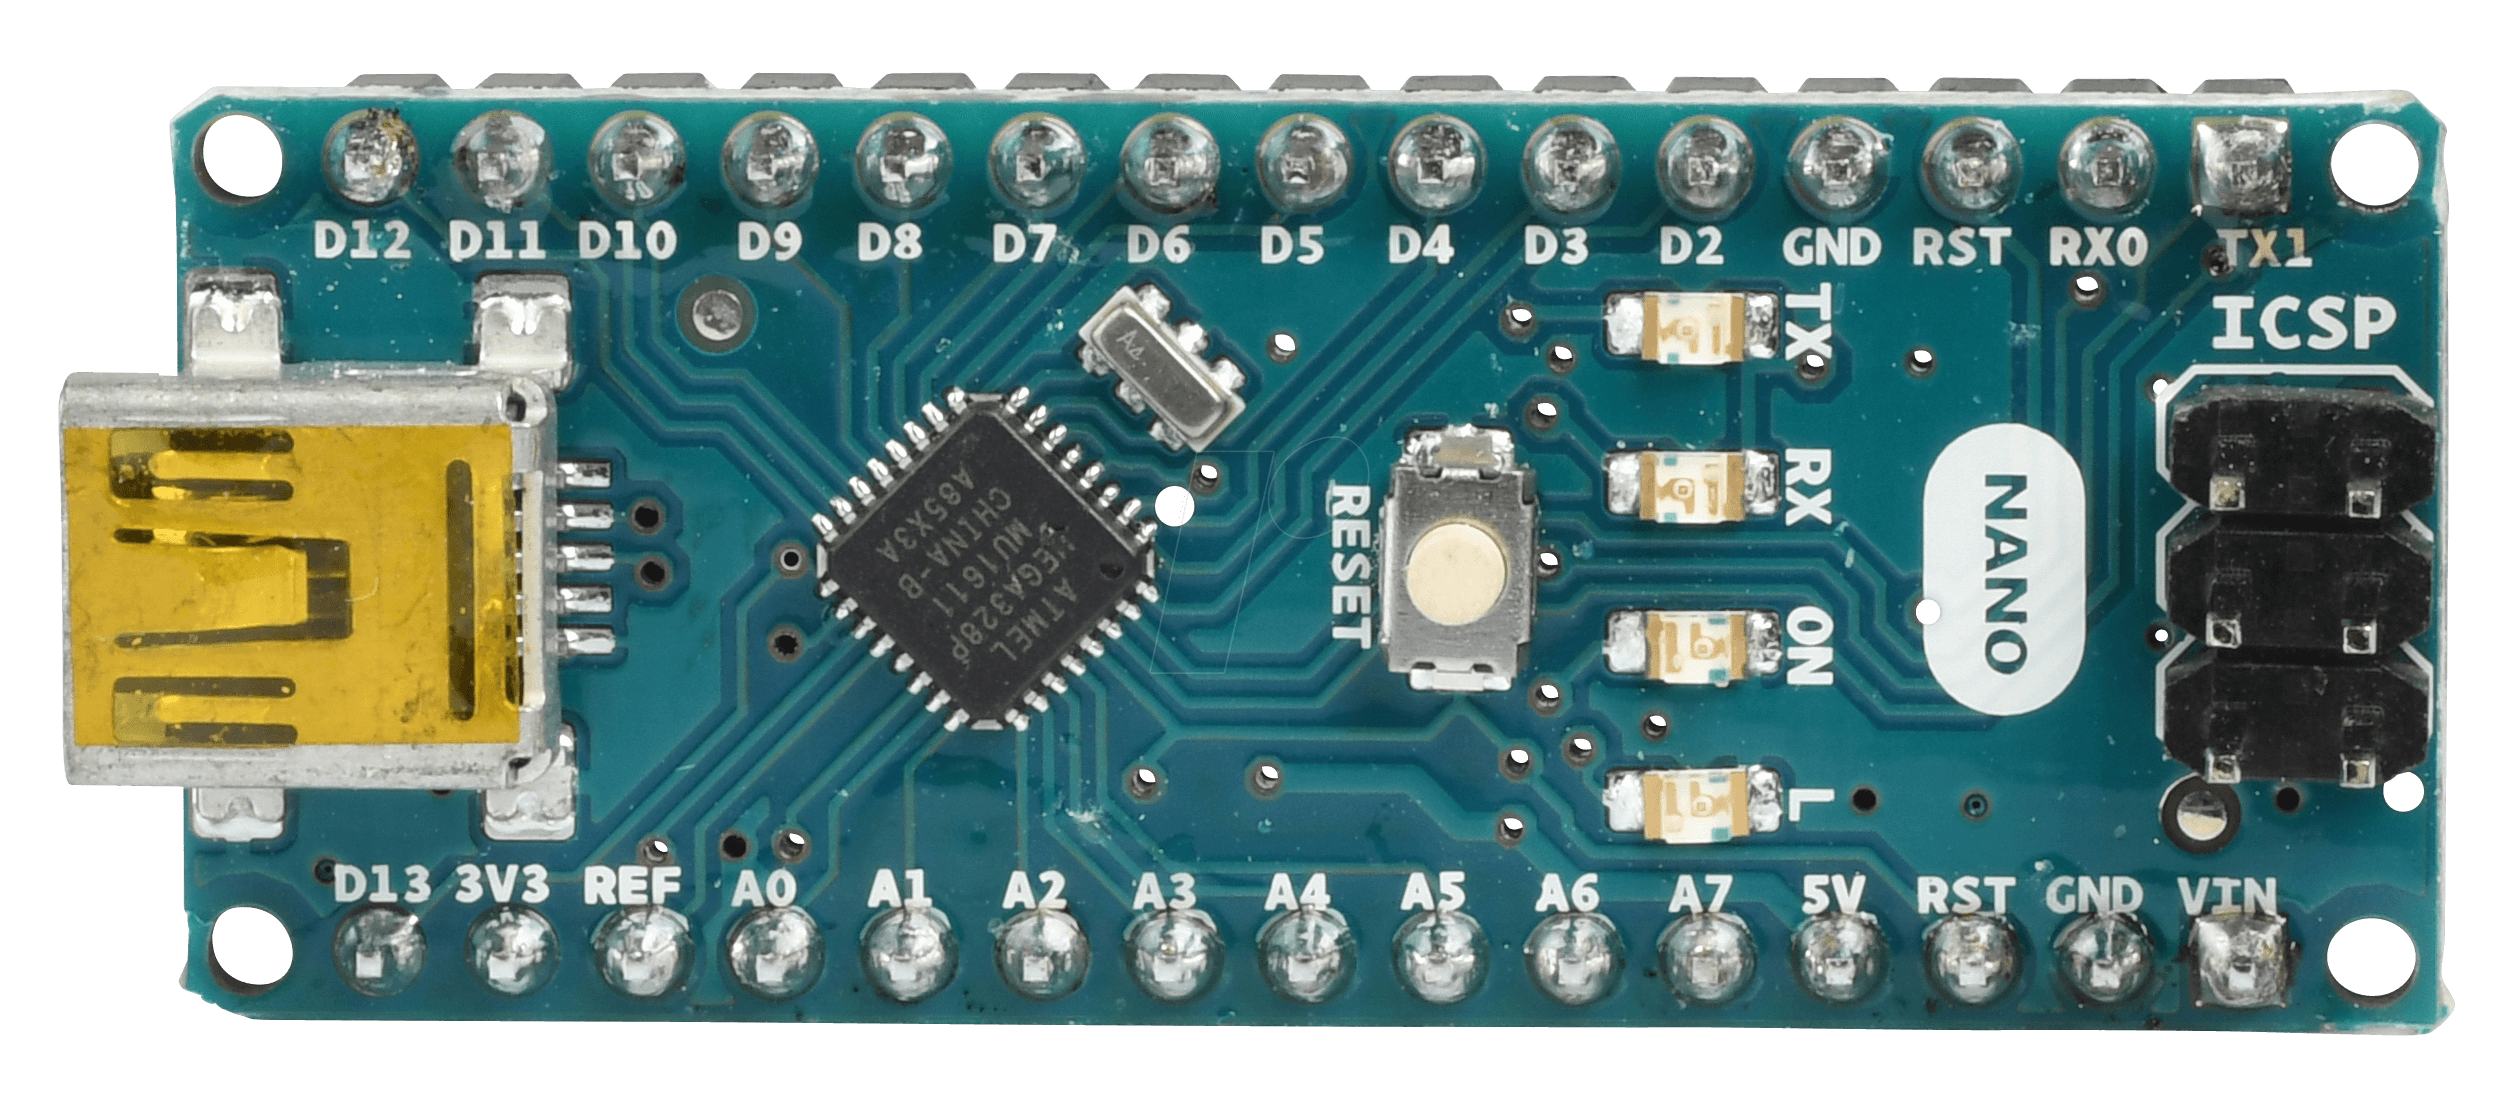
\includegraphics[width=0.5\textwidth]{arduinonano.png}
	\caption{Vista superior de um Arduino Nano. Fonte:store.arduino.cc}
\end{figure}
\begin{figure}[H]
	\centering
	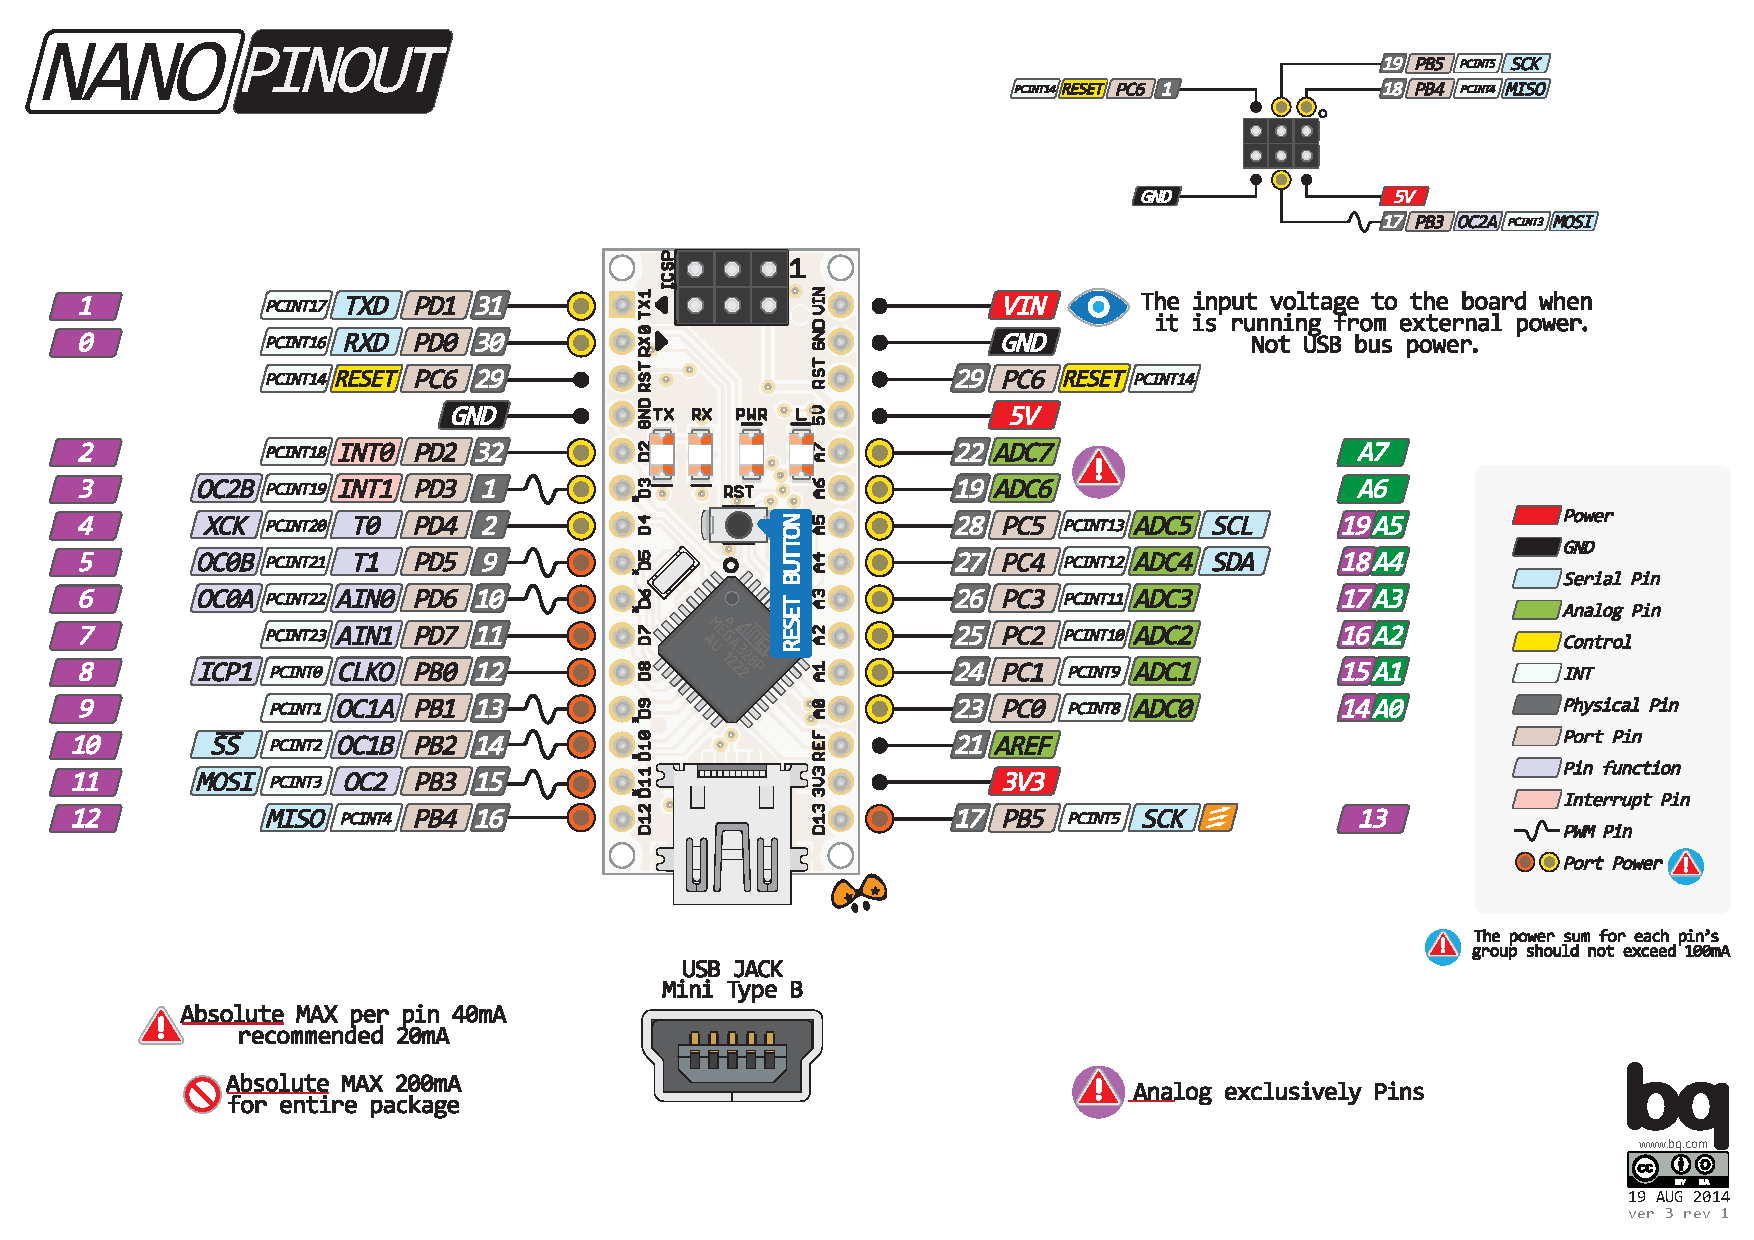
\includegraphics[width=0.9\textwidth]{nano.pdf}
	\caption{Infográfico pinagem arduino e suas funções}
\end{figure}

\section{Controlador para motores TB6612FNG}\label{TB6612FNG}
Segundo o \textit{datasheet} disponibilizado pela empresa Toshiba, o \textbf{TB6612FNG} é um driver que pode controlar até dois motores de corrente continua. Com o total de 16 pinos, dois pinos são entrada, sendo eles \textbf{IN1} e \textbf{IN2} dos quais podem ser usados para controlar uma dentre as quatro modos de operação !!CW, CCW, short-brake, and stop!!. Quatro pinos de saída -\textbf{A01, A02, B02 e B01}- para os motores, podendo ser controlados separadamente. A velocidade de cada motor pode ser controlado por um sinal de \textbf{PWM} nos seus respectivos pinos \textbf{PWMA} e \textbf{PWMB}, o driver possui um pino \textbf{STBY}, abreviação do inglês \textit{standby} que pode ser traduzido para espera, ou seja, modo de espera, para retira-lo do modo de espera deve-se colocar a tensão deste pino em alta (\textit{HIGH}). O pino \textbf{VCC} é destinado a suprir a demanda de energia do driver, sendo operacional com tensões de 2,7 até 5,5 volts de corrente continua, já o pino \textbf{VM} é destinado a suprir a demanda de energia dos motores, tendo seu limite máximo de 15 volts em corrente continua. 

!!Board comes with all components installed as shown. Decoupling capacitors are included on both supply lines. All pins of the TB6612FNG are broken out to two 0.1" pitch headers; the pins are arranged such that input pins are on one side and output pins are on the other.
Note: If you are looking for the SparkFun Motor Driver with headers, it can be found here or in the Recommended Products below.!!

\begin{figure}[H]
	\centering
	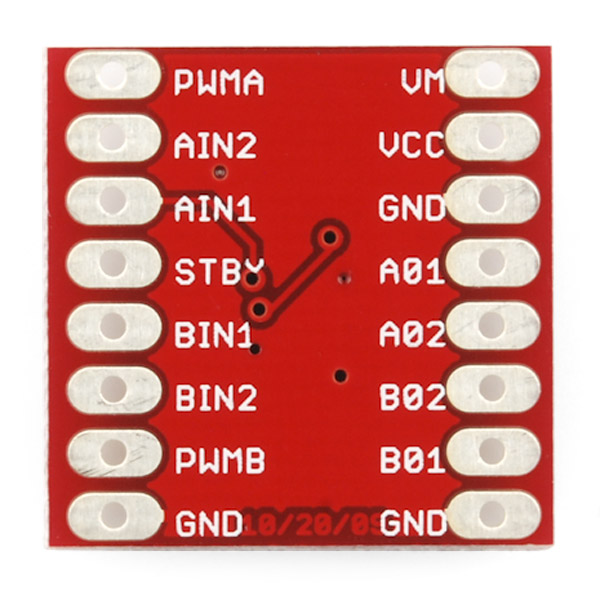
\includegraphics[width=0.5\textwidth]{inferiorTB6612FNG.jpg}
	\caption{Vista inferior do driver TB6612FNG com os rótulos de seus respectivos pinos. Fonte:www.sparkfun.com}
\end{figure}

Para entendermos o funcionamento básico do controlador \textbf{TB6612FNG} a tabela a seguir descreve as possibilidades de configuração para o controlador, considerando que o pino \textit{\textbf{STBY}} e \textit{\textbf{PWM}} estão em alto(\textit{high}) em todos os casos, ou seja, os casos de \textit{\textbf{STBY/PWM}} baixos(\textit{low}) não estarão presentes na tabela.
\begin{table}[!h]
	\renewcommand{\arraystretch}{1.3}
	\centering
	\begin{tabular}{|c|c|c|c|c|}
		\hline
		\textbf{IN1} & \textbf{IN2} & \textbf{OUT1} & \textbf{OUT2} & \textbf{MODO} \\ \hline
		    ALTO     &     ALTO     &     BAIXO     &     BAIXO     & FREADA RÁPIDA \\ \hline
		   BAIXO     &     ALTO     &     BAIXO     &     ALTO      &   ROTAÇÃO 1   \\ \hline
		    ALTO     &    BAIXO     &     ALTO      &     BAIXO     &   ROTAÇÃO 2   \\ \hline
		   BAIXO     &    BAIXO     &   DESLIGADO   &   DESLIGADO   &    PARADO     \\ \hline
	\end{tabular}
	\caption[Tabela verdade controle motor]{Lista de funcionamento e atuação de um motor DC para o controlador TB6612FNG.}
	\label{Tab:TB6612FNG}
\end{table}
Como podemos ver na tabela verdade do controlador \textbf{TB6612FNG} podemos ver o funcionamento igual a de uma ponte-H, com as duas entradas carregadas não ah corrente de saída em ambas as portas, alternando a corrente entre as portas \textbf{IN1} e \textbf{IN2} mudamos o sentido de rotação do motor e por ultimo com as duas entradas sem carga as portas \textbf{OUT} não apresentam saída de tensão, sendo assim controlando as portas \textbf{IN} com o Arduino podemos controlar o sentido de rotação de cada um dos motores, visto que o \textbf{TB6612FNG} pode controlar até dois motores.

\section{Sensor Óptico TCRT1000}\label{TCRT1000}
O sensor óptico modelo \textbf{TCRT1000}, segundo a documentação da empresa \textit{Vishay} obtidas no sitio \textit{www.vishay.com}, é um conjunto de um emissor infravermelho com um fototransistor, inseridos em um invólucro de chumbo para bloquear a luz visível evitando erros nas leituras no fototransistor um sensor de pequenas dimensões medindo apenas 7mm x 4mm x 2.5mm e pode ser utilizado como mostrado na imagem \ref{fig:lateralmodu}, em robô com dois sensores para cada roda.
\begin{figure}[H]
	\centering
	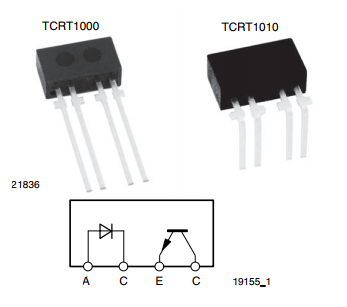
\includegraphics[width=0.5\textwidth]{TCRT1000.jpg}
	\caption{Sensor óptico TCRT1000. Fonte:www.vishay.com}
\end{figure}
\begin{figure}[H]
	\centering
	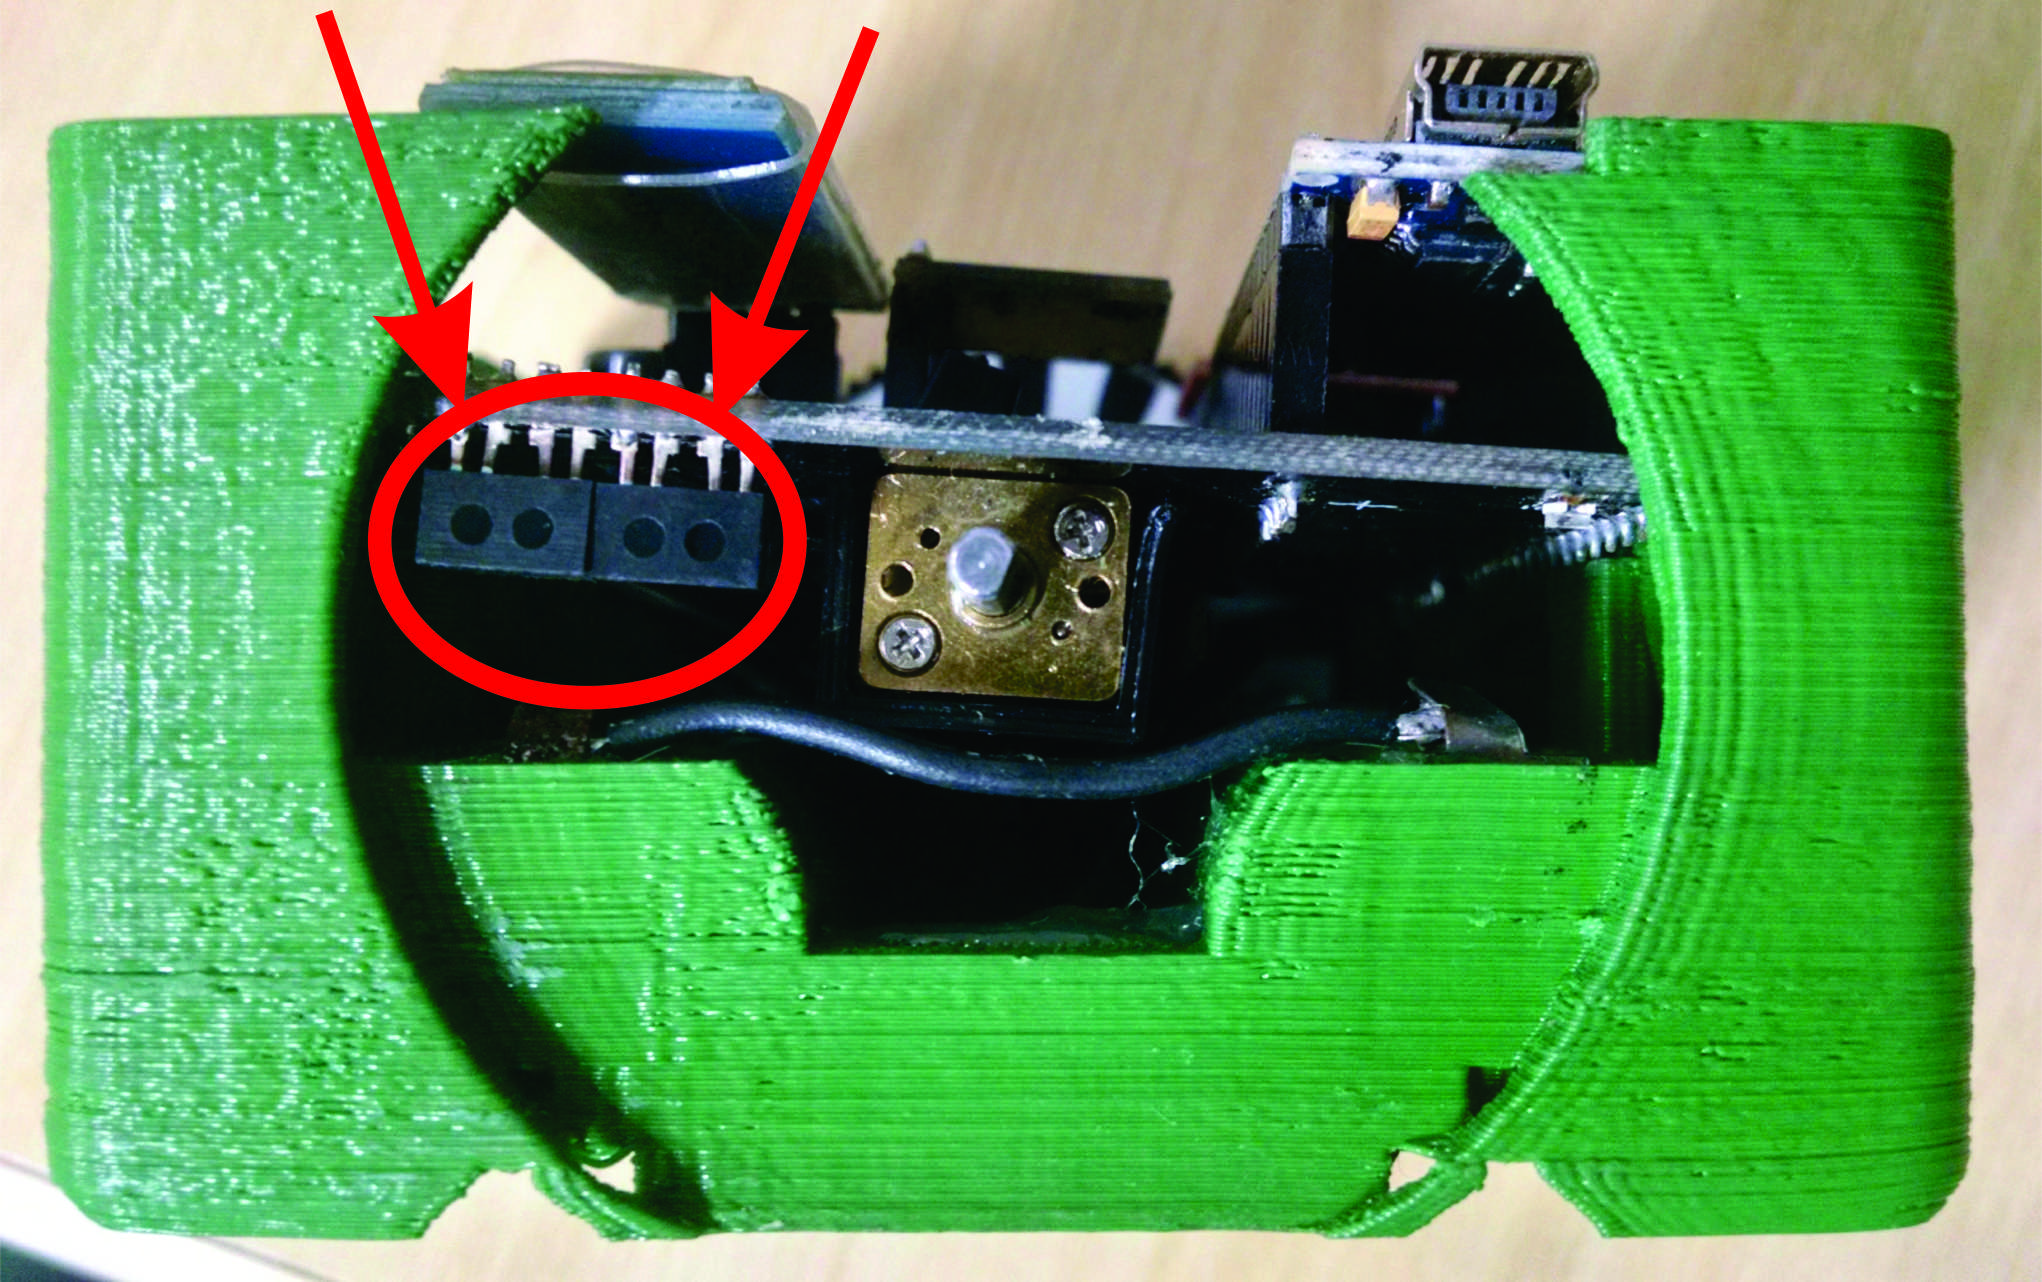
\includegraphics[width=0.5\textwidth]{lateralmodu.jpg}
	\caption{Vista lateral do robô Modu sem a roda, carcaça verde feita em impressora 3D, dois sensores ópticos e eixo de motor}
	\label{fig:lateralmodu}
\end{figure}

\section{Roda}\label{roda}
O robô Modu possui apenas um par de rodas de !!XX mm!! e uma faixa de marcadores, utilizados juntamente com os sensores ópticos \ref{TCRT1000} transformando todo o conjunto em um encoder \ref{encoder} descrito na próxima sessão, tendo 17 marcadores brancos e 17 marcadores preto totalizando 34 marcadores como pode ser visto na figura \ref{fig:roda34marc}.
\begin{figure}[H]
	\centering
	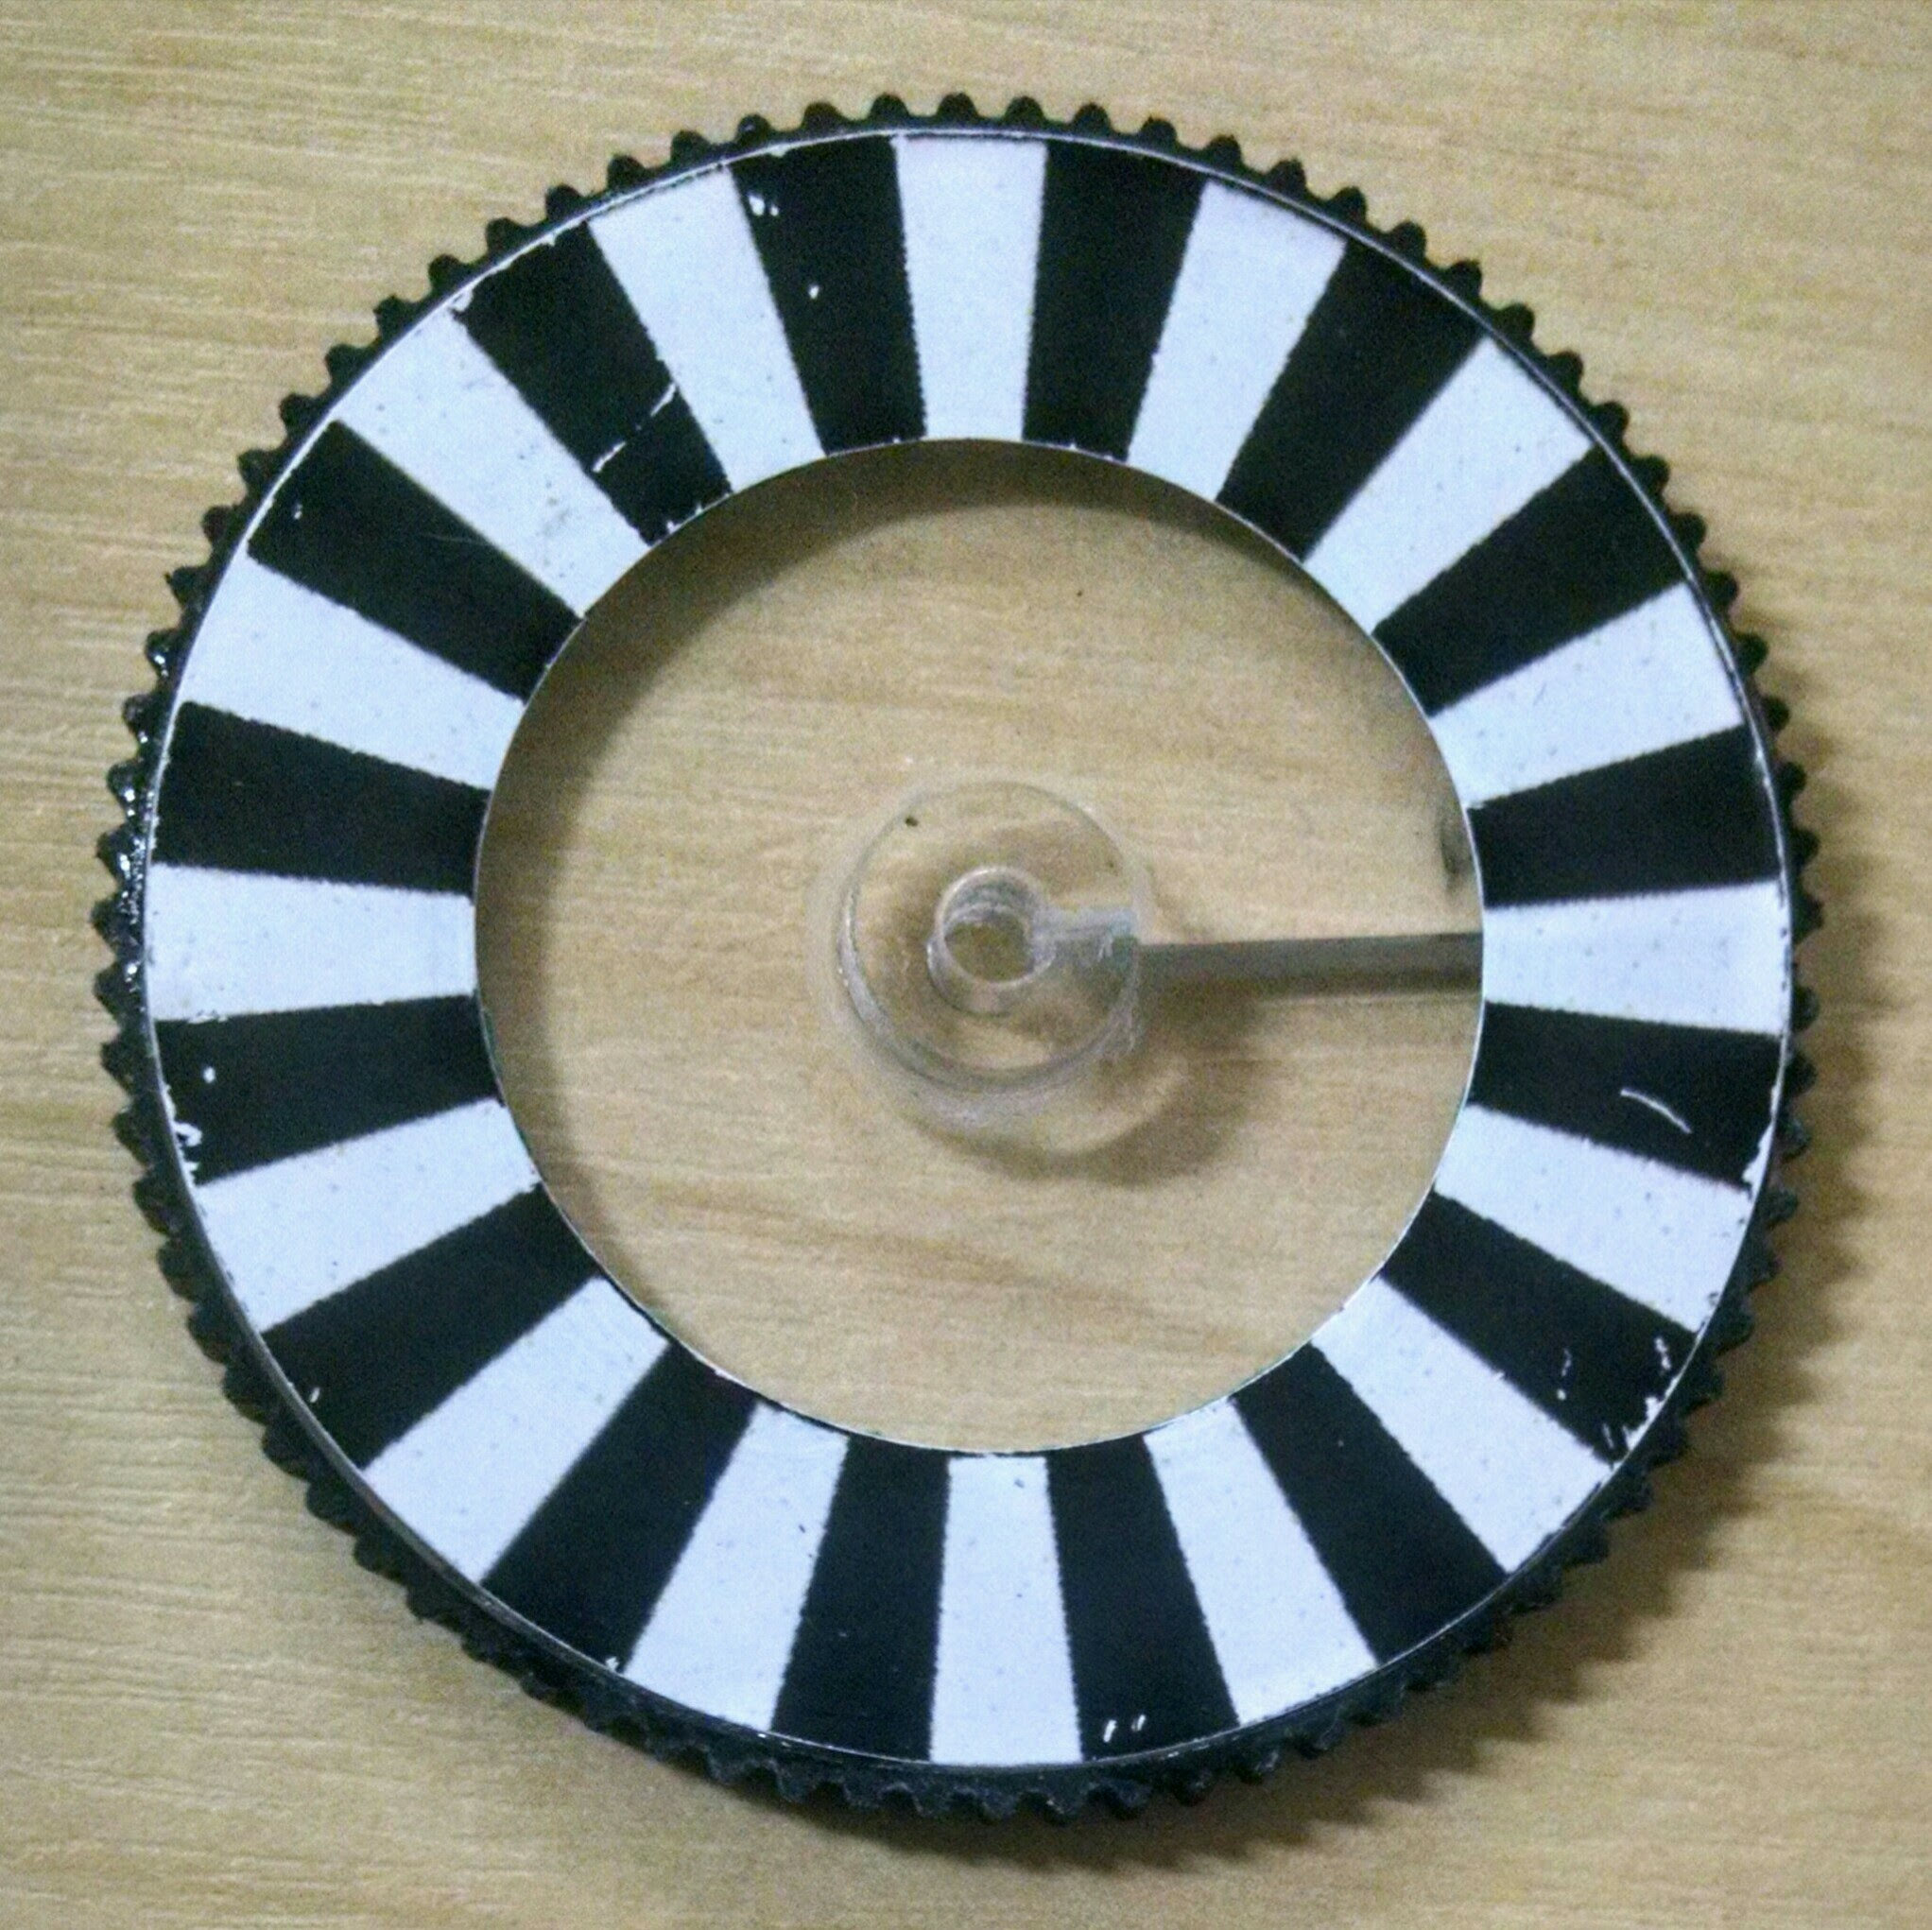
\includegraphics[width=0.5\textwidth]{roda32marc.jpg}
	\caption{Roda com fita de 32 marcadores}
	\label{fig:roda32marc}
\end{figure}
\begin{figure}[H]
	\centering
	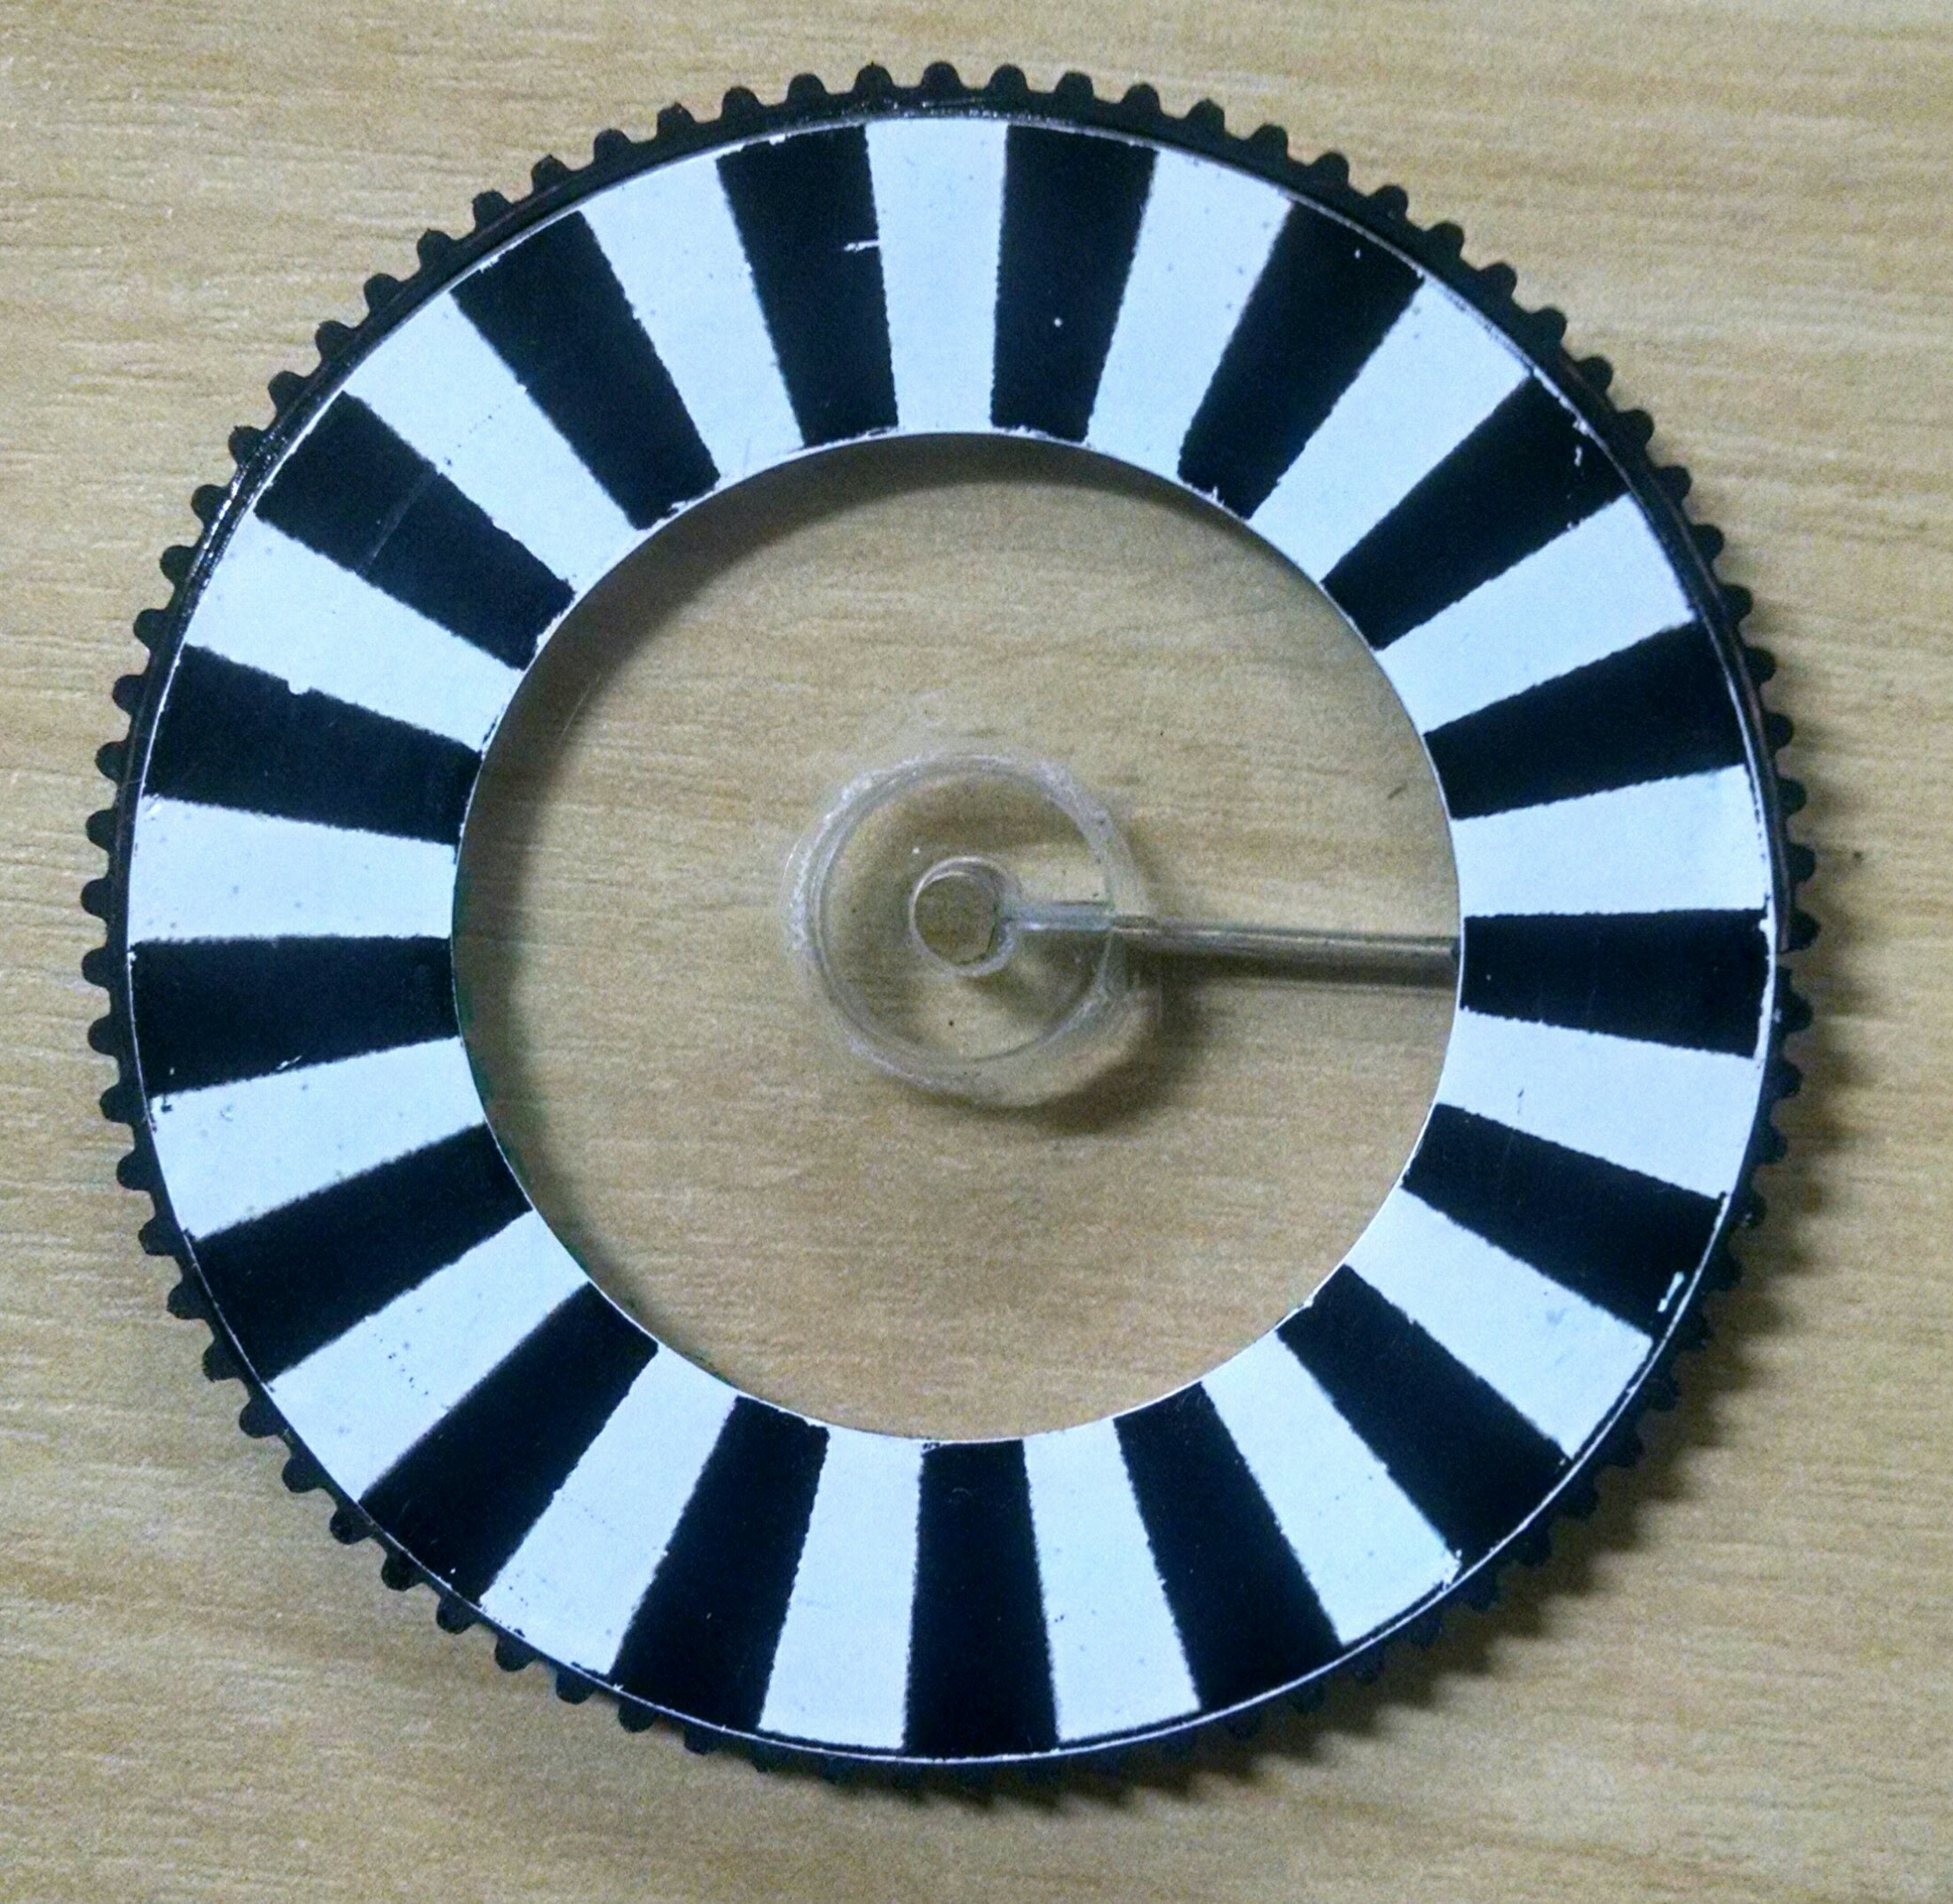
\includegraphics[width=0.5\textwidth]{roda34marc.jpg}
	\caption{Roda com fita de 34 marcadores}
	\label{fig:roda34marc}
\end{figure}
\begin{figure}[H]
	\centering
	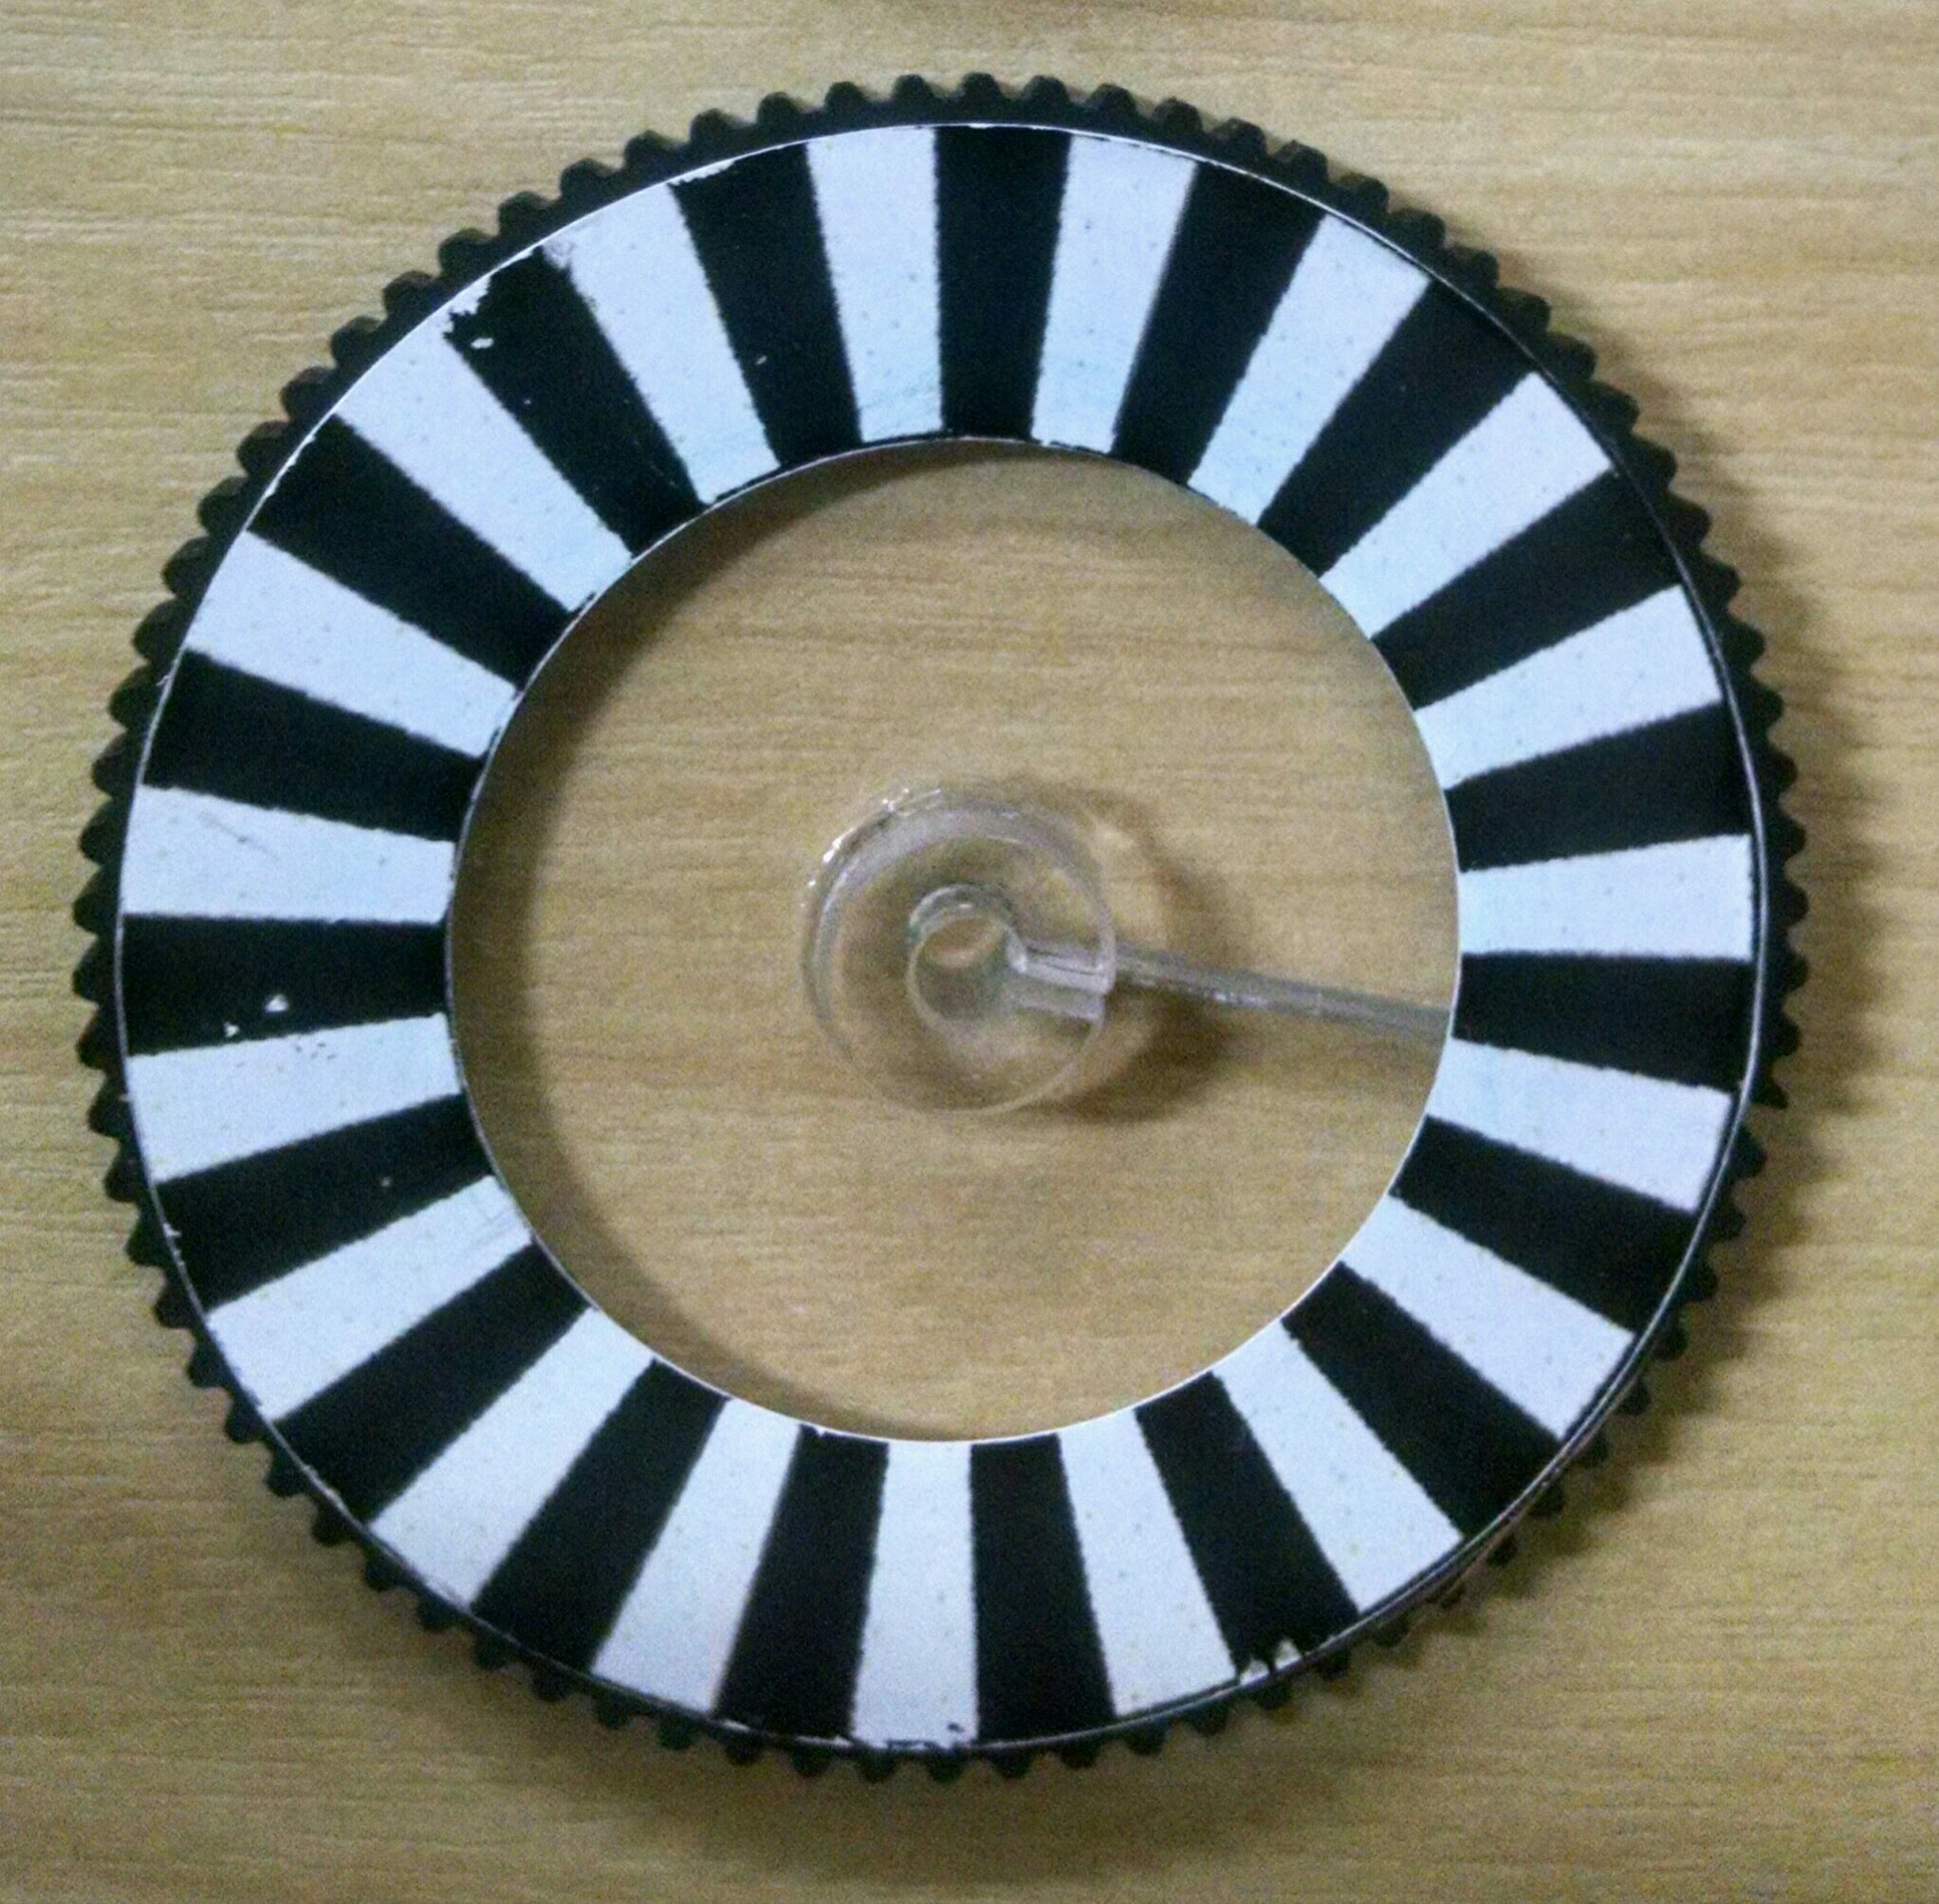
\includegraphics[width=0.5\textwidth]{roda38marc.jpg}
	\caption{Roda com fita de 38 marcadores}
	\label{fig:roda38marc}
\end{figure}

\section{Encoder}\label{encoder}
Em resumo NC Braga descreve um encoder como um componente formado por transistores precisos que pode converter movimento linear ou angular em sinais digitais, dos quais geralmente são utilizados para determinas a posição\cite{braga2009funcionam}, velocidade e em alguns casos dependendo da configuração do encoder pode-se também determinar a direção de rotação do sistema. 

\section{Bluetooth HC-06}\label{bthc06}
O modulo foi utilizado para comunicação sem fio entre o robô e o computador, as informações são trocadas utilizando do protocolo \textit{Serial}, o alcance do módulo segue o padrão da comunicação bluethooth, aproximadamente 10 metros, o suficiente, visto que o campo não passa pouco dos dois metros. Uma característica deste modelo (HC-06) possui apenas o modo \textit{slave} neste modo é apenas permitido receber conexão de outros dispositivos, ou seja, não permite que este modelo busque e solicite conexão com outros dispositivos, assim como ocorre com fones de ouvido e caixas de som.
\begin{figure}[H]	
	\centering
	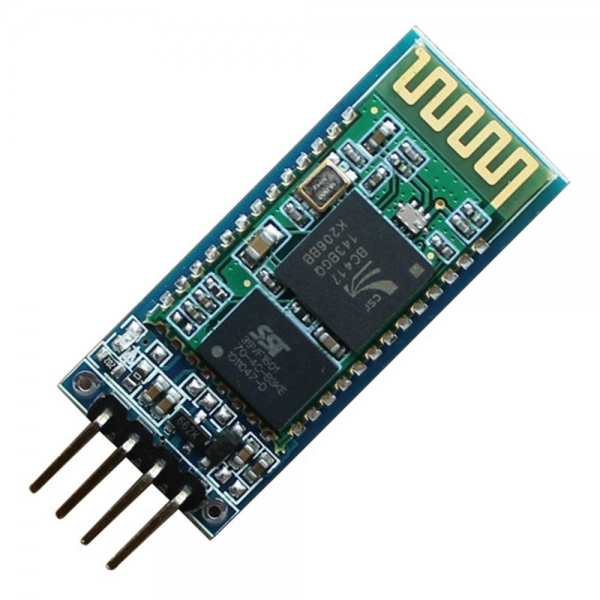
\includegraphics[width=0.5\textwidth]{BTHC06.jpg}
	\caption{Vista superior de um componente bluetooth modelo HC-06. Fonte:http://buildbot.com.br}
\end{figure}

\chapter{Ambiente de desenvolvimento}
Este capítulo aborda as ferramentas utilizadas para o desenvolvimento da programação dos robôs jogadores. O sistema operacional escolhido foi o Ubuntu Gnome 17.04 64-bit, por ser uma distribuição linux o Ubuntu já possui os drivers USB para comunicação a placas de teste, a utilizada no projeto foi a placa Arduino Nano 328, com o driver USB, como o FTDI. Sera descrito também neste capítulo a instalação e configuração dos softwares: IDE Arduino, IDE Clion 2017.1 e PlatformIO.

\section{Arduino IDE}\label{arduinoide}
======== https://www.arduino.cc/en/main/software ===
O Arduino 1.8.3(IDE) é um software open-source para desenvolvimento de programas para Arduino. A utilização deste software torna fácil escrever códigos e subir(upload) para a placa. O Arduino IDE tem suporte para Windows, Mas OS e para Linux. Ambiente foi desenvolvido em Java baseado no Processing e outros softwares open-source, com a utilização da IDE qualquer placa Arduino pode ser utilizada com poucas configurações.

\subsection{Intalação}
Na pagina oficial de download https://www.arduino.cc/en/Main/Software foi realizado o download conforme o sistema operacional, neste caso, Linux x64, ao selecionar o download é possível fazer uma doação para os desenvolvedores da IDE, visto que é um projeto open-source e software livre, não tendo fins lucrativos, o mesmo depende dessa colaboração da comunidade para permanecer ativo e continuar expandido. Então realizado o download da versão atual, neste momento a versão 1.6.10 para linux.

\begin{figure}[H]	
	\centering
	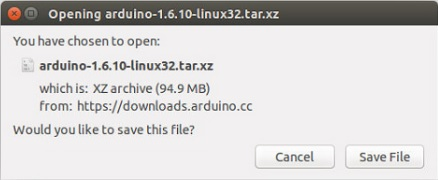
\includegraphics[width=0.5\textwidth]{dlArduino.jpg}
	\caption{Titulo.}
\end{figure}
Ao finalizar o download do arquivo compactado, sera necessário descompactar em um diretório desejado, este ainda não sera o diretório de instalação. 
\begin{figure}[H]	
	\centering
	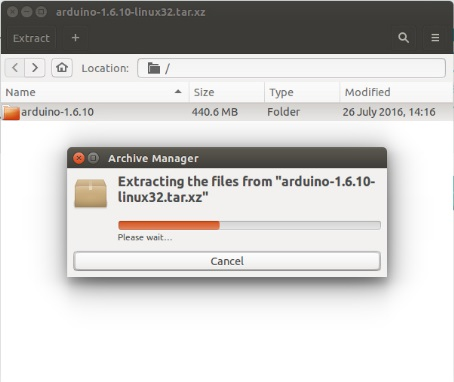
\includegraphics[width=0.5\textwidth]{unrarArduino.jpg}
	\caption{Titulo.}
\end{figure}
Abrindo o terminal navegue pelos diretórios utilizando o comando ‘CD’ até o diretório arduino-1.6.x o qual foi criado ao descompactar o arquivo. Execute então o arquivo ‘intall.sh’ utilizando o comando: 
\begin{lstlisting}
./install.sh
\end{lstlisting}
O processo de instalação é rápido, um novo ícone foi criado na área de trabalho.
\begin{figure}[H]	
	\centering
	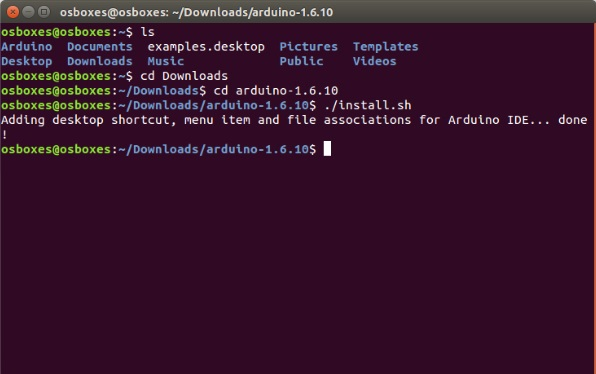
\includegraphics[width=0.5\textwidth]{installArduino.jpg}
	\caption{Titulo.}
\end{figure}

\section{Clion 2017.1}
====== https://www.jetbrains.com/clion/ =======
CLion é uma IDE multi-plataforma, criada pela empresa JetBrains para desenvolvimento de softwares nas linguagens C e C++, uma ferramenta poderosa. Suporte as linguagens nativas C e C++, incluindo C++11, C++14, libc++ e mais. A ferramenta desenvolvimento conta com ótimos recursos tais como: navegação, geração de código, gerenciamento de bibliotecas entre outros.

\subsection{Instalação}
Na página oficial de download do Clion ``https://www.jetbrains.com/clion/download/\#\=linux" foi realizado o download do arquivo ``CLion-*.tar.gz" da versão compatível com o sistema operacional. Descompacte o arquivo ``CLion-*.tar.gz", neste projeto foi descompactado no diretório /opt, sendo assim foi utilizado o seguinte comando para descompactar direto no diretório desejado.
\begin{lstlisting}
sudo tar xf CLion-*.tar.gz -C /opt/
\end{lstlisting}
Ao finalizar a descompactação, novamente navegue até o diretório /bin, diretório este que se encontra junto aos arquivos descompactados, utilizando o comando: 
\begin{lstlisting}
cd /opt/CLion-*/bin
\end{lstlisting}
Execute o arquivo clion.sh que se encontra dentro do subdiretório /bin, com o comando:
\begin{lstlisting}
./clion.sh
\end{lstlisting}

\section{PlatformIO}
Diferente microcontroladores normalmente exigem diferentes ferramentas de desenvolvimento, para o Arduino temos a Arduino IDE. Outros usuários preferem ferramentas com auxílios. Tais ambientes de desenvolvimentos como o Eclipse, o qual trás recursos que ajudam a gerenciar seus projetos, bibliotecas e funções de autocompletar. As vezes é um pouco difícil manter-se na linha com diferentes microcontroladores e ferramentas. Então o ecossistema (como é chamado pelos seus desenvolvedores) open-source do PlatformIO junta tudo em uma única ferramenta. Sendo uma ferramenta multiplataforma podendo ser instalada nos sistemas operacionais Linux, Windows e MAC, dá suporte ao compilação para mais de 200 placas de teste, com mais de 15 plataformas de desenvolvimento e 10 frameworks, cobrindo então as placas mais populares do mercado, fazendo o trabalho duro de organização de centenas de projeto e bibliotecas que podem ser incluídas no projeto.

\subsection{Instalação}
A instalação ou atualização no MAC e Linux é feita pelo terminal de um modo muito fácil, apenas utilizando o comando(sudo pode ser requerido): 
\begin{lstlisting}
python -c "$(curl -fsSL https://raw.githubusercontent.com/platformio/platformio/master/scripts/get-platformio.py)"
\end{lstlisting}

\section{Iniciando um novo projeto}
Para criar um novo projeto primeiramente devemos abrir a IDE Clion, deve-se criar um novo projeto na linguagem C++ clicando no File, New Poject então em Create. Ao finalizar a criação do novo projeto, abra as opções de configurações utilizando o atalho de teclado ``Ctrl + Alt + S" clique na aba ``Plugins” no campo de texto procure por Arduino, conforme a figura abaixo. Caso não seja localizado no repositório local clique em ``Search in repositories” para procurar nos repositórios da JetBrains.
\begin{figure}[H]	
	\centering
	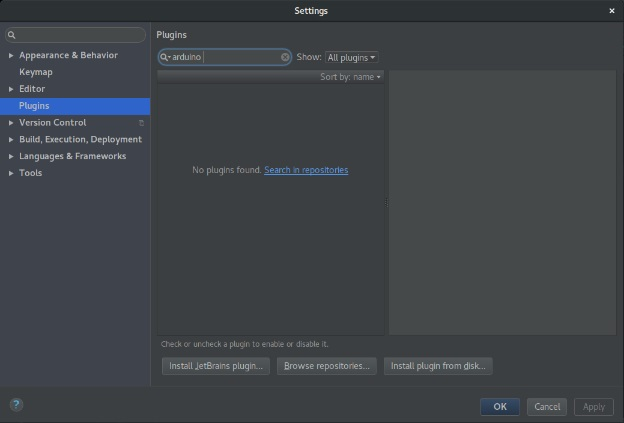
\includegraphics[width=0.5\textwidth]{pluginClion.jpg}
	\caption{Titulo.}
\end{figure}
\begin{figure}[H]	
	\centering
	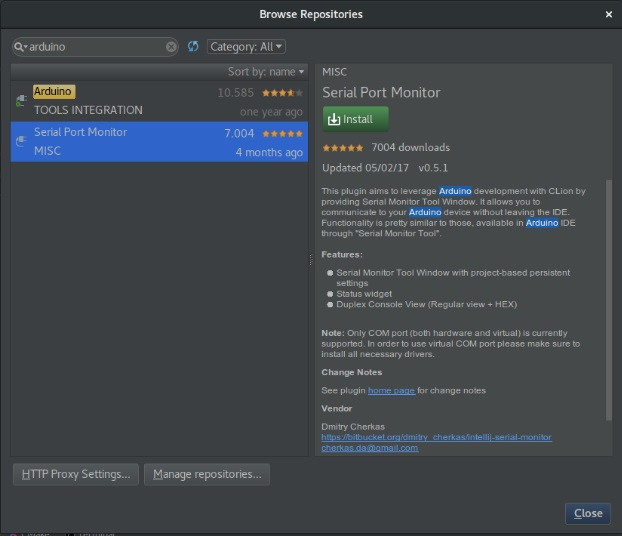
\includegraphics[width=0.5\textwidth]{pluginClion2.jpg}
	\caption{Titulo.}
\end{figure}
Após o final da instalação dos dois plugins reinicie o CLion para os plugins venham funcionar. Com a IDE aberta, no terminal, navegue com o comando ``CD" até o diretório do projeto o qual acabou de ser criado. Neste projeto foi criado a pasta TCCTerceira no diretório de projetos do CLion o qual se encontra na home do linux.
\begin{lstlisting}
cd /home/kelvimro/CLionProjects/TCCTerceira
\end{lstlisting}
Ainda no terminal é utilizado o comando ``platformio” com a opção ``boards”, este comando lista as placas de teste suportadas pelo PlatformIO.
\begin{lstlisting}
platformio boards
\end{lstlisting}
Ao localizar a placa desejada na lista, Arduino Nano processador Atmel 328, a qual foi escolhida para ser utilizada no desenvolvimento dos robôs de futebol do time UFMS-CPCX.
\begin{figure}[H]	
	\centering
	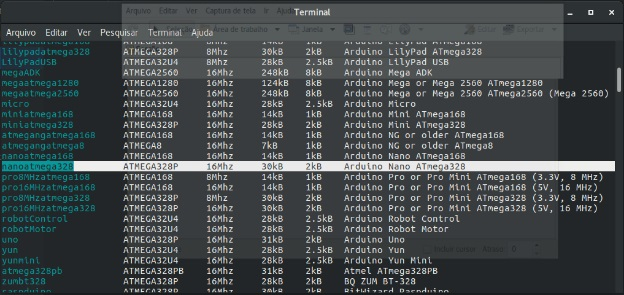
\includegraphics[width=0.5\textwidth]{boardPlatformio.jpg}
	\caption{Titulo.}
\end{figure}
Localizado e copiado o nome da placa ``nanoatmega328”, utilize o comando ``platformio” com as opções de ``init” para iniciar/instalar os recursos necessários no projeto,  a opção ``ide” deve-se ser utilizada o parâmetro ``clion" indicando que utilizamos o framework para trabalhar junto a IDE do Clion, sendo assim o comando completo utilizado foi:
\begin{lstlisting}
platformio init --ide clion --board nanoatmega328
\end{lstlisting}
\begin{figure}[H]	
	\centering
	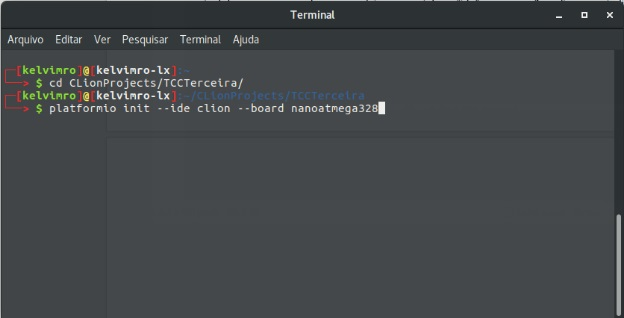
\includegraphics[width=0.5\textwidth]{initPlatformio.jpg}
	\caption{Titulo.}
\end{figure}
Finalizando a inicialização do PlatformIO será nescessário recarregar o arquivo CMake. Para isso clique com o botão direito do mouse em cima do nome do projeto(TCCTerceira) e em seguida em ``Reload CMake Project".
\begin{figure}[H]	
	\centering
	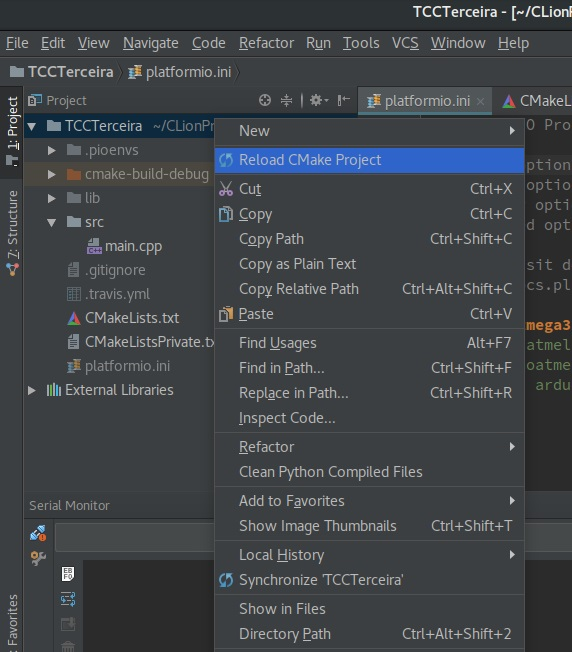
\includegraphics[width=0.5\textwidth]{reloadCmake.jpg}
	\caption{Titulo.}
\end{figure}
O PlatiformIO requer que as classes, assim como a Main.cpp, deve estar dentro da subpasta ``src" pois a ferramenta é configurada nativamente para buscar e compilar os códigos que ali estão. Na classe Main.cpp deve-se fazer o importe da biblioteca ``Arduino.h" por meio do ``\#include" a qual é a sintaxe para importar em C.
\begin{lstlisting}
#include <Arduino.h>
\end{lstlisting}
O código a seguir foi utilizado para teste de compilação e funcionamento do ambiente como um todo no fim da configuração. O programa tem a função básica, de piscar o led embutido na placa do arduino (LED\_BUILTIN) ou seja o pino da porta 13, ficando 1 segundo acesso e 1 segundo apagado.

\begin{lstlisting}
#include <Arduino.h>
void setup() {
// inicializa o pino digital LED_BUILTIN como saida.
pinMode(LED_BUILTIN, OUTPUT);
}

// Função loop do arduino
void loop() {
digitalWrite(LED_BUILTIN, HIGH);   // liga o LED 
delay(1000);                       // espera um segundo
digitalWrite(LED_BUILTIN, LOW);    // desliga o LED
delay(1000);                       // espera um segundo
}
\end{lstlisting}

Compilando o código utilizando Ctrl + F9 ou clicando no ícone no canto superior direito
\begin{figure}[H]	
	\centering
	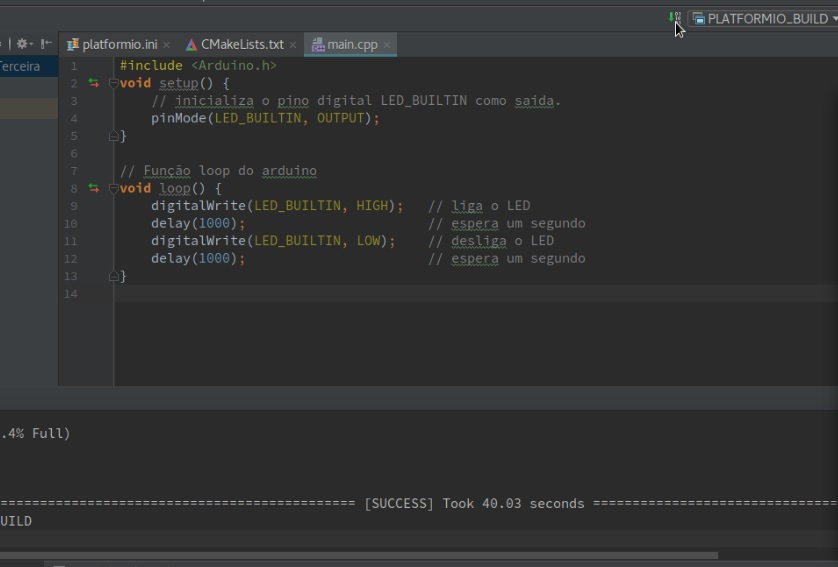
\includegraphics[width=0.5\textwidth]{buildClion.jpg}
	\caption{Titulo.}
\end{figure}
Ao receber a mensagem de ``SUCCESS" na aba ``Messages", indica que o ``build" ou seja, a compilação do programa foi concluída com exito.
No fim a compilação (build) é hora de subir(upload) do código para a placa arduino mudando para opção PLATFORMIO\_UPLOAD ( na caixa de seleção no canto superior direito) e clicando no ícone ``PLAY" verde.
\begin{figure}[H]	
	\centering
	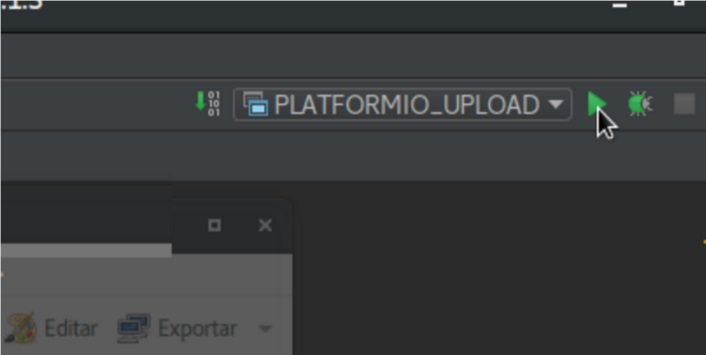
\includegraphics[width=0.5\textwidth]{upload.jpg}
	\caption{Titulo.}
\end{figure}
Aguarde a próxima mensagem de sucesso, a qual indicando que o programa já foi completamente enviado a placa, então o código já rodando.
ATENÇÃO: Algumas distribuições podem solicitar a permissão de administrador para ter acesso ao dispositivo USB antes de fazer o upload do código. O privilégio pode ser concedido com a utilização do comando:
\begin{lstlisting}
sudo chmod 777 /dev/ttyUSB0
\end{lstlisting}
Ps.: O numero “0” em ttyUSB0 deve ser trocado conforme a porta ao qual o dispositivo foi conectado.

Ps2.: Em algumas distribuições as permissões devem ser dadas sempre o dispositivo for conectado/reconectando.
Finalizando assim as configurações do ambiente de desenvolvimento, que foi utilizado para gerenciar e editar os códigos neste trabalho de conclusão.

\chapter{Controle Bluetooth}
Um simples projeto foi desenvolvido também em Arduino. O projeto tem a finalidade de ser um controle BT(Bluetooth) com um Joystick, utilizado para controlar as direções do robô. 
O joystick, um dos componentes do controle, nada mais é que dois potenciômetros, um potenciômetro para os valores do eixo X e outro para os valores do eixo Y. 
O controle possui um componente BT para estabelecer uma troca de dados junto ao robô, o qual também possui seu componente BT, o qual será explicado no capítulo\ref{bthc05}.
O código atualizado pode ser encontrado no link: https://github.com/kelvimro/TCCTerceira/blob/master/lib/ControleBT/controleBT.cpp 
O controle tem o intuito de simular os comandos que são gerados pela inteligência artificial no software que é responsável pelas táticas e movimento dos jogadores durante uma partida.
Os comandos podem variam entre -100 até 100, tendo um valor para cada motor, ou seja cada computação realizada pela inteligência artificial é enviado dois números inteiros, onde o primeiro número é destinado ao motor esquerdo e o segundo ao direito.
Utilizando-se da função map() a qual proporciona os valores do potenciômetro - dos quais variam entre 0 a 1023 - aos valores válidos para o robô.
\begin{lstlisting}
if (cmdX >= 0 && cmdX <= 501) cmdX = map(cmdX, 0, 501, -100, 0);
else cmdX = map(cmdX, 502, 1023, 0, 100);
if (cmdY >= 0 && cmdY <= 509) cmdY = map(cmdY, 0, 509, -100, 0);
else cmdY = map(cmdY, 510, 1023, 0, 100);
\end{lstlisting}
O potenciômetros Y, o qual vai representar os valores de potência, em posição neutra (sem ação do controlador) encontra-se com valor analógico de 509, então mapeado para 0, ou seja, não há potência requerida.
Ao movimentar o joystick para frente, aumenta-se o valor analogio do potenciômetro até o máximo de 1023 que após ter seu valor mapeado representa o valor 100.
Movimentando o joystick para trás, os valores analógicos lido diminuem até 0, denotando o valor -100. 
\begin{lstlisting}
if (cmdY >= 0 && cmdY <= 509) cmdY = map(cmdY, 0, 509, -100, 0);
else cmdY = map(cmdY, 510, 1023, 0, 100);
\end{lstlisting}
Valores positivos no eixo Y indicam que o movimento solicitado é para frente, enquanto os valores negativos representam movimento para trás.
O potenciômetros X, o qual vai representar os valores da diferença entre os motores. Em sua posição neutra tem o valor analógico lido de 502, representando 0\% de diferença entre os motores. Afim de facilitar a compreensão chamaremos de A o motor do lado esquerdo e de B o motor do lado direito. Então ao movimentar o joystick para a esquerda o valor analógico lido diminui até 0, resultando no valor de -100, movimentando o joystick para a direita aumentando o valor analógico lido até 1023 que representa o valor 100. 
\begin{lstlisting}
if (cmdX >= 0 && cmdX <= 501) cmdX = map(cmdX, 0, 501, -100, 0);
else cmdX = map(cmdX, 502, 1023, 0, 100);
\end{lstlisting}
No eixo X os valores negativos indicam que o motor A tem de se movimentar X\% mais lento em relação ao motor B, fazendo o movimento de curva para o lado de A. Já com os valores positivos de X indica que o motor B deve ser X\% mais lento q o A fazendo a curva para o lado B.

\section{Blutooth HC-05}\label{bthc05}


\chapter{Interrupções}
O processador do Arduino Nano, o qual foi utilizado neste projeto é do modelo Atmega328 e nesta seção discorreremos sobre o funcionamento da interrupção neste processador, utilização no projeto, exemplos e !!efeitos colaterais!!.
Em sua maioria os processadores possuem interrupções dos quais permitem executar algo após determinado evento externo, sendo chamado de interrupções externas. Nas referencias online presentes no site oficial do Arduino, para mais informações a cerca de interrupções é indicado as notas de Nick Gammon!!(https://gammon.com.au/interrupts)!!, de um modo didático e simples ele faz um paralelo ao cotidiano, ao fazer o jantar e ter de cozinhar as batatas, é colocado um despertador com o tempo de 20 minutos, indo faze outra atividade durante o tempo de cozimento, ao despertar o alarme vc ``interrompe" sua atividade e então termina o jantar. Apesar do exemplo utilizado ser quase uma mudança de estado, não é recomendado invocar funções grandes e complexas pois além de sair da linha principal de execução, as funções não contem argumentos, utilizamos então variáveis do tipo voláteis. Logo recomenda-se as interrupções para trocas de \textit{flag}, disparo de funções emergenciais, contagens precisas entre outros a interrupção é o ``botão vermelho", veremos a seguir que \textit{reset} é a interrupção de maior prioridade.

\section{Rotinas de serviço de interrupção (ISR)}\label{isr}
As rotinas de serviço de interrupção conhecidas pela sigla ISR que vem do inglês \textit{Interruption Service Rotines} é uma rotinha a qual se encontra fora da função \textbf{loop}, ou sejá, é uma função a qual será executada quando ocorrer uma interrupção, interrompendo a execução do código \textbf{loop} onde quer que ele esteja, retornando ao ponto de ``pausa" ao fim da ISR. Algo de suma importância é citado por Simon Monk em seu livro, Programação com Arduino vol. 2 \begin{quote}``Quando uma ISR está sendo executada, as interrupções são automaticamente desligadas. Isso evita a confusão que poderia ser causada se as ISRs interrompessem umas as outras."\end{quote}
Ou seja, enquanto uma ISR estiver ativa outras não serão executadas, exceto uma interrupção de maior prioridade como o \textit{reset}.

\section{Modos de Interrupção}\label{modointerrupcao}
Os chamados modos de interrupção é como gatilho, irá disparar a ISR, ou seja, uma ISR é uma função a ser executada sempre quando o gatilho é acionado. O Atmega328 possui quatro modos de interrupção, são eles: \\
\textbf{LOW} - Dispara uma interrupção continuamente enquanto o pino selecionado estiver em nível baixo (\textit{low}).\\
\textbf{RISING} - Dispara uma interrupção sempre que o pino passar de baixo (\textit{low}) para alto (\textit{high}).\\
\textbf{FALLING} - Dispara uma interrupção sempre que o pino passar de alto (\textit{high}) para baixo (\textit{low}).\\
\textbf{CHANGE} - Dispara uma interrupção sempre que o pino mudar de nível, em ambos os sentidos.\\
Vale ressaltar que o modelo Arduino Due tem um quinto modo de interrupção, o \textit{HIGH}.\\
\textbf{HIGH} - Dispara uma interrupção continuamente enquanto o pino estiver em nível alto (\textit{high}), assim como o modo \textit{LOW}.

\section{Interrupção no Atmega328}\label{interrupcao328}
Assim como em outros processadores o Atmega328 possui sua lista de interrupções, logo a baixo podemos ve-la em ordem de prioridade, tendo em primeiro lugar -maior prioridade- a interrupção de \textit{reset}.

\begin{table}[!h]
	\renewcommand{\arraystretch}{1.3}
	\centering
	\begin{tabular}{|c|cc|}
		\hline
		1  &                      Reset                      &  \\ \hline
		2  &     External Interrupt Request 0  (pin D2)      &     (INT0\_vect)     \\ \hline
		3  &     External Interrupt Request 1  (pin D3)      &     (INT1\_vect)     \\ \hline
		4  & Pin Change Interrupt Request 0 (pins D8 to D13) &    (PCINT0\_vect)    \\ \hline
		5  & Pin Change Interrupt Request 1 (pins A0 to A5)  &    (PCINT1\_vect)    \\ \hline
		6  & Pin Change Interrupt Request 2 (pins D0 to D7)  &    (PCINT2\_vect)    \\ \hline
		7  &           Watchdog Time-out Interrupt           &     (WDT\_vect)      \\ \hline
		8  &         Timer/Counter2 Compare Match A          & (TIMER2\_COMPA\_vect) \\ \hline
		9  &         Timer/Counter2 Compare Match B          & (TIMER2\_COMPB\_vect) \\ \hline
		10 &             Timer/Counter2 Overflow             &  (TIMER2\_OVF\_vect)  \\ \hline
		11 &          Timer/Counter1 Capture Event           & (TIMER1\_CAPT\_vect)  \\ \hline
		12 &         Timer/Counter1 Compare Match A          & (TIMER1\_COMPA\_vect) \\ \hline
		13 &         Timer/Counter1 Compare Match B          & (TIMER1\_COMPB\_vect) \\ \hline
		14 &             Timer/Counter1 Overflow             &  (TIMER1\_OVF\_vect)  \\ \hline
		15 &         Timer/Counter0 Compare Match A          & (TIMER0\_COMPA\_vect) \\ \hline
		16 &         Timer/Counter0 Compare Match B          & (TIMER0\_COMPB\_vect) \\ \hline
		17 &             Timer/Counter0 Overflow             &  (TIMER0\_OVF\_vect)  \\ \hline
		18 &          SPI Serial Transfer Complete           &   (SPI\_STC\_vect)    \\ \hline
		19 &                USART Rx Complete                &   (USART\_RX\_vect)   \\ \hline
		20 &           USART, Data Register Empty            &  (USART\_UDRE\_vect)  \\ \hline
		21 &               USART, Tx Complete                &   (USART\_TX\_vect)   \\ \hline
		22 &             ADC Conversion Complete             &     (ADC\_vect)      \\ \hline
		23 &                  EEPROM Ready                   &   (EE\_READY\_vect)   \\ \hline
		24 &                Analog Comparator                & (ANALOG\_COMP\_vect)  \\ \hline
		25 &         2-wire Serial Interface  (I2C)          &     (TWI\_vect)      \\ \hline
		26 &           Store Program Memory Ready            &  (SPM\_READY\_vect)   \\ \hline
	\end{tabular}
	\caption[Lista de interrupções]{Lista de interrupções para o chip processador Atmega328. Fonte: gammon.com.au/interrupts}
	\label{Tab:interrupcoes}
\end{table}

Como podemos na tabela acima as interrupções externas nomeadas de \textbf{INT0\_vect} e \textbf{INT1\_vect} que correspondem aos pinos digitais 2 e 3 respectivamente, no Arduino Nano(os pinos de interrupção podem mudar de acordo com a placa) sendo as maiores prioridades seguidas do \textit{reset}, aproveitamos para observar as interrupções de 7 a 17, as quais são interrupções de tempos e a interrupção de prioridade 25 a qual é a interrupção para uso da interface serial.

\section{Utilizando interrupção no Arduino}\label{usointerrupcao}
Nesta seção foi como exemplos os códigos utilizados no robô no desenvolvimento do trabalho, conforme visto na seção anterior \ref{interrupcao328} os pinos de interrupção são os pinos digitais 2 e 3. Declaramos então no código as variáveis das quais irá representar os pinos, utilizando o código.
\begin{lstlisting}
const int encodPinA1 = 2;                       // encoder A pino 2
const int encodPinB1 = 3;                       // encoder B pino 3
\end{lstlisting}
Dentro da função \textit{setup} !!intanciamos!! os pinos como \textit{INPUT} pois estes pinos farão a entradas de informação ao pino de interrupção.
\begin{lstlisting}
pinMode(encodPinA1, INPUT);
pinMode(encodPinB1, INPUT);
\end{lstlisting}
Segundo as refecias disposta na documentação do site oficial do Arduino temos três sintaxes diferentes para acoplar\//iniciar, porem dentre elas apenas uma é recomendada pelos desenvolvedores, sendo assim foi utilizado a sintaxe recomendada.
\begin{lstlisting}
attachInterrupt(digitalPinToInterrupt(pin), ISR, mode);
\end{lstlisting}
A função \textbf{digitalPinToInterrupt(pin)} é utilizada para traduzir o pino digital para o numero especifico da interrupção.
ISR \ref{isr} é o nome da função a ser chamada quando a interrupção ocorrer, lembrando que esta função não deve conter argumentos.
\textit{Mode} define o modo de quando a interrupção deve disparar, conforme descrito na seção \ref{modointerrupcao}.
Seguindo então a sintaxe recomendada para iniciar nossa interrupção com o pino e função desejada.
\begin{lstlisting}
attachInterrupt(digitalPinToInterrupt(encodPinA1), rencoderA, CHANGE);
attachInterrupt(digitalPinToInterrupt(encodPinB1), rencoderB, CHANGE);
\end{lstlisting}
Como pode ser visto no código acima, a função com nome de \textbf{rencoderA} (ISR) será executada sempre que seu valor do pino \textbf{encodPinA1} mudar, pois seu modo foi defino como \textit{CHANGE}, o mesmo acontece com o pino \textbf{encodPinB1} chamando sua respectiva ISR nomeada como \textbf{rencoderB}. 
\begin{lstlisting}
	void rencoderA() {
	countA++;
	}
	void rencoderB() {
	countB++;
	}
\end{lstlisting}
Do mesmo modo que podemos acoplar uma interrupção a um pino especifico, também podemos desacopla-lo utilizando o código a seguir sempre que achar necessário.
\begin{lstlisting}
detachInterrupt(digitalPinToInterrupt(encodPinA1));
detachInterrupt(digitalPinToInterrupt(encodPinB1));
\end{lstlisting}
O código exemplificado acima tem a função de desativar a interrupção do pino \textbf{encodPinA1} e do pino \textbf{encodPinB1} exclusivamente.

Existe um modo alternativo de ativar e ativar\//desativar as interrupções, mas estas funções ativam\//desativam todas a interrupções - exceto \textit{rest} -
\begin{lstlisting}
interrupts();		// Ativa interrupções
noInterrupts();		// Desativa interrupções
\end{lstlisting}
Lembrando que ao desativando as interrupções utilizando-se da função acima citada, as interrupções citadas na tabela \ref{Tab:interrupcoes}como a \textit{Serial} também são desativada. Sendo muito útil quando nos trechos de códigos sensíveis ao tempo, no código a seguir desativamos as interrupções para evitar que os valores da variável contadora sejam alterados durante a execução, evitando erros de leitura quanto as velocidades das rodas.
\begin{lstlisting}
	noInterrupts();				// Desarma interrupts
	calibA.push(countA);		// Adiciona a ultima contagem a fila de amostras
	countA = 0;					// Zera contadores de marcos do encoder
	calibMillis = millis();		// Zera o contador de tempo
	interrupts();				// Arma interrupsts
\end{lstlisting}

\chapter{Controlador PID}\label{pid}
== https://www.citisystems.com.br/controle-pid/ ===
Neste capítulo, explanarei sobre o controle PID -que é abreviatura para Proporcional, Integral e Derivativo- e como utiliza-lo em aplicações de controle que requerem um controle de precisão. Começaremos pelo exemplo onde um carro tenta manter uma distancia X do carro da frente.

\section{P - Proporcional}
Ao tentar manter uma distancia X o carro de trás deve acelerar proporcionalmente quando o carro da frente acelerar e começar a distanciar, tentando alcançar o mesmo. No entanto, caso o carro de trás venha acelerar mais que o carro da frente a distancia será menor que a desejada, X, então a nova correção é frear para aumentar a distancia buscando a distancia desejada de X. Novamente caso a correção, que desta vez é a frenagem(desaceleração), for muito, a sua distancia se será superior a distancia desejada de X, então novamente terá de acelerar. Isso ocorrera indefinitivamente caso a aceleração não proporcional não esteja correta, ou seja, acelerando de mais e freando de menos e não atingindo o ponto alvo(\textit{set point}). Então esta aceleração é chapada de ganho ou proporcional(P) em um controle PID.

\section{I - Integral}
A integral, neste exemplo dos carros, seria como recuperar a distancia X a cada instante, caso o veiculo da frente venha a acelerar, o veiculo de trás acelera gradualmente afim de atingir a distancia X com mais suavidade, este procedimento pode ser comparado a integral de um controle PID.

\section{D - Derivativo}
A derivada é utilizada para eliminar erros acumulados na integral, neste exemplo dos carros, seria quando o carro de trás percebe que a distancia desce ou decresce muito rapidamente em relação a desejada X, deixando as correções da integral ainda mais suaves, diminuindo a oscilação das correções em volta do Setpoint.

\section{Utilização do PID}
O controle do tipo PID foi empregado para controlar a velocidade da roda mais rápida em relação a mais lenta, como pode ser visto até o então, o controle PID se utiliza de dados obtidos durante a sua execução, no caso deste trabalho o tempo de um ciclo foi de 200 milissegundos(ms), ou seja, a cada 200 ms o controle obtém a velocidade de rotação de ambas as rodas por meio do encoder \ref{encoder} utilizando a velocidade do motor mais lento como \textit{set point} do motor mais rápido, calculando a proporcional, a integral e derivando, utilizando o resultado como o novo valor do PWM do motor mais rápido o deixando com a velocidade de rotação mais próxima do motor de referencia.

\subsection{Problemas no ciclo}
Durante o emprego do controle PID para equalizar as velocidades dos motores foi percebido que o tempo de ciclo para o controle se tornar eficiente é superior o intervalo de comandos recebidos pelo computador de controle o qual envia novos comandos a cada 200ms. O controle do tipo PID não consegue equalizar as velocidades na primeira correção, então ao se aproximar da segunda ou terceira correção o robô recebe a próxima instrução mudando todas as referencias de velocidades.

\subsection{Problemas devido interrupções}
Como pode ser visto o encoder \ref{encoder} é o conjunto da roda \ref{roda} provida de marcadores e  dos sensores ópticos \ref{tcrt1000}, para realizar a contagem de marcadores os sensores ópticos estão conectados nos pinos digitais 2 e 3, se utilizando da função de interrupção para contagem dos marcadores e determinas as velocidades, veremos no próximo capitulo, mais precisamente na seção de rotinas de interrupção \ref{isr}, que ao gerar uma interrupção todo o sistema ``para" temporariamente, trazendo discrepância nas contagens devido a sobreposição de interrupções.
Concluindo então que a utilização de controle do tipo PID do modo implementado não é recomendado.

\chapter{Controle por pesos}
Um controle por peso é de simples funcionamento, cada motor tem seu peso o qual é multiplicado pelo seu PWM solicitado pelo computador controlador dos robôs, com a diferença dos pesos os motores mesmo com potencia real diferente tendem a rodarem com uma velocidade parecida. Para atribuir valores aos pesos, foram feito os !!X!! passos começando com coleta de amostras, calculando a média das amostras adquiridas e então calculando os pesos.

\section{Coleta de amostras - getAmostras(int \_PWM)}\label{getamostras}
Foi desenvolvido um método chamado \textbf{getAmostras(int \_PWM)} tendo como argumento o PWM desejado para coleta de amostras.
O método então coleta o numero de amostras determinado na variável \textbf{NUM\_AMOSTRA} de escopo global como pode ser visto na linha 2 do código abaixo, também podemos verificar a variável \textbf{CALIBMILLIS} a qual determina intervalo de tempo para cada amostras. Afim de evitar erros na contagem devido a interrupções \ref{isr} as contagens são executadas separadamente, ou seja, primeiro é colhido as amostras do motor A e depois colhida as amostras do motor B.
\begin{lstlisting}
	// Numero de amostras para a media movel
	int NUM_AMOSTRA = 15;
	// Tempo de coleta de amostras
	const int CALIBMILLIS = 1000;
\end{lstlisting}
Sendo usado a configuração acima, a contagem de impulsos gerados pelo encoder \ref{encoder} é realizada durante um intervalo de 1000 milissegundos, gerando então uma amostra. 
Logo abaixo o código da função na integra, a variável \textit{print} é do tipo \textit{String} e de escopo global, utilizada para armazenar informações a serem impressas posteriormente.  
\begin{lstlisting}
void getAmostras(int _PWM) {
	print = "PWM =\t";
	print += _PWM;
						 // https://www.arduino.cc/en/Reference/NoInterrupts
	noInterrupts();									// Desativa interrupções
	print += "\nA:\n";
	PWM_valA = _PWM;				// PWM_valA é o PWM do motor A de 0 a 255
	PWM_valB = 1;					// PWM_valA é o PWM do motor A de 0 a 255
	motorRefresh();
	countB = countA = 0;
	static double calibMillis;				   	// calibMillis timer de loop
	calibMillis = millis();
	interrupts();									// Reativa intrrupções
	while (PWM_valA >= 5) {
		for (int i = 0; i < NUM_AMOSTRA; ++i) {// Controla numero de amostras
				  	// Enquanto encoder conta durante CALIBMILLIS, faça nada ;)
			while ((millis() - calibMillis) <= CALIBMILLIS) {}
			noInterrupts();         				   // Desarma interrupts
			calibA.push(countA);// Adiciona a ultima contagem a fila de amostras
			print += countA;
			print += "\n";
			countA = 0;                  // Zera contadores de marcos do encoder
			calibMillis = millis();				    // Zera o contador de tempo
			interrupts();              						// Arma interrupsts
		}
		PWM_valA = PWM_valB = 2;				// Reduz vel. mas mantem sentido
		motorRefresh();
	}
	noInterrupts();										// Desativa interrupções
	// Set PWM - config inicial
	print += "\nB:\n";
	PWM_valA = 1;
	PWM_valB = _PWM; 			 	   // PWM_valA é o PWM do motor A de 0 a 255
	motorRefresh();
	countB = countA = 0;
	calibMillis = millis();
	interrupts();
	while (PWM_valB >= 5) {
		for (int i = 0; i < NUM_AMOSTRA; ++i) {
							// Enquanto conta durante CALIBMILLIS, faça nada :)
			while ((millis() - calibMillis) <= CALIBMILLIS) {}
			noInterrupts();								 // Desarma interrupts
			calibB.push(countB);
			print += countB;
			print += "\n";
			countB = 0;				 	// Zera contadores de marcos do encoder
			calibMillis = millis();
			interrupts();									// Arma interrupsts
		}
		PWM_valA = PWM_valB = 2;
		motorRefresh();
	}
	Serial.print(print); 	   			// Imprime o conteudo da variavel print
	print = " ";			 							// Esvazia variavel print
	if (processMedia()) {}    // Invoca o metodo responsavel por calcular a média
}
\end{lstlisting}
Como podemos ver no código acima a linha 1 é a declaração do método de retorno \textit{void}, sem retorno. Excluindo as linhas da variável \textit{print} da explicação visto que a mesma é apenas impressão de informações, podemos observar nas linhas 5, 18, 29 e 42 o comando \textbf{noInterrupts();} e nas linhas 13, 24, 37 e 48 o comando \textbf{interrupts();} ambos explicados na sessão \ref{usointerrupcao}. As linhas 12, 23, 36 e 47 pode ser visto o comando \textbf{millis();} este tem como retorno o numero em milissegundos dês de que a placa Arduino começou a rodar o programa, sendo assim nas linhas citadas é como se marcasse o horário da execução na quele instante e gravados na variavel \textbf{calibMillis}.
Os PWM são utilizados como critérios de parada da função \textit{while} nas 14 e 38, sendo alterados apenas quando o \textit{for} da linha 15 obter o numero de amostras determinados em \textbf{NUM\_AMOSTRA}.
As duas estruturas de repetição \textit{while}, nas linhas 17 e 41 é utilizadas como uma espera, a fim de evitar a função \textbf{delay();} a qual se utiliza de interrupções \ref{Tab:interrupcoes} para executar a espera, sendo assim não há execução de nenhum código até que o tempo atual \textbf{millis()} subtraindo o ultimo tempo atual -anotado na linha 12- seja maior que o tempo de coleta determinado na variável \textbf{CALIBMILLIS}, após decorrido tempo de \textbf{CALIBMILLIS} em milissegundos, é desativado as interrupções na linha 18 afim de não aumentar a contagem de marcadores, esta contagem a qual é salva na variável \textbf{contA}, após desativar as interrupções é adicionado a uma estrutura de fila chamada \textbf{calibA} a ultima contagem de \textbf{countA} conforme a linha 19 logo após salvar a ultima contagem este contador é zerado na linha 22, anotando-se o novo tempo atual na linha 23 e reativando as interrupções na linha 24, este processo será executado até obter o numero desejado de amostras devido a função \textit{for} da linha 15, ao fim, obtendo o numero total de amostras os PWMs do motor A e B são setados para 2, afim de para-los então chamado o metodo \textbf{motorRefresh();} o qual simplesmente atualiza os valores de PWM nos motores como pode ser visto no código abaixo, finalizando a coleta de amostras para o motor A.
\begin{lstlisting}
void motorRefresh() {
	PWM_valA *= pesoA;
	PWM_valB *= pesoB;
	PWM_valA = int(PWM_valA);
	PWM_valB = int(PWM_valB);
	analogWrite(PWMA, PWM_valA);
	analogWrite(PWMB, PWM_valB);
}
\end{lstlisting}
O mesmo processo ocorre para aquisição de amostras para o motor B entre as linhas 29 e 52, desativando interrupções, determinando o valor do PWM de B para o PWM a ser testado, zerando os contadores, salvando o tempo atual, fazendo as esperas no \textit{while} assim como ocorreu no motor A.
Ao final da coleta das amostras de ambos os motores, antes de retornar a função, um método chamado \textbf{processMedia()} é invocado para calcular a média das 15 amostras de cada motor.

\section{Média de amostas - processMedia()}\label{processmedia}
A função cujo tem por finalidade computar a média para cada roda, sempre será executada que a função \textbf{getAmostras(int)} for invocada, utilizando-se das amostras já obtidas conforme a sessão \ref{getamostras}.
\begin{lstlisting}
boolean processMedia() {
	static double _soma;
	_soma = 0;
	static double _med;
	_med = 0;
	static int _mark;
	_mark = 0;
	print = "\nMédia\t";
	while (!calibA.isEmpty()) {
		_soma += calibA.pop();
		_mark++;
	}
	_med = _soma / _mark;
	mediaA.push(_med);
	print += _med;                   			         // Imprime média de A
	_soma = 0;
	_med = 0;
	_mark = 0;
	while (!calibB.isEmpty()) {
		_soma += calibB.pop();
		_mark++;
	}
	_med = _soma / _mark;
	mediaB.push(_med);
	print += "\t";         			       // Imprime indicadores e média de B
	print += _med;
	delayMicroseconds(999);
	Serial.println(print);	
	return true;
}	
\end{lstlisting}
A função começa declarando três (\textbf{\_soma, \_med e \_mark}) variáveis locais, pois são utilizadas apenas dentro da função, as variáveis são utilizadas para auxiliar nos cálculos, declaradas como estáticas afim de economizar memória, utilizando-se da mesma variável sempre que a função for chamada. Ao estanciar as variáveis nas linhas 2, 4 e 6 e zeradas nas linhas 3, 5 e 7 inicia-se o processo de calculo da média propriamente dita na linha 9 onde o critério de parada da estrutura de repetição \textit{while} é a função \textit{.isEmpty()} uma função disponível da estrutura de dados da variável \textbf{calibA} e \textbf{cablibB} que são do tipo fila, esta função -\textit{.isEmpty()}- retorna verdadeiro (\textit{true}) caso a fila esteja vazia, sendo assim enquanto a fila \textbf{calibA} não estiver vazia soma-se o atual valor de \textbf{\_soma} ao valor retirado da fila utilizando a função \textit{.pop()} conforme a linha 10, então incrementando 1 o valor de \textbf{\_mark} na linha 11, a variável \textit{\_mark} tem por finalidade contar o numero exato de amostras retiradas da fila, ou seja, sempre uma amostra for retirada da fila é incrementado em um ao marcador. Assim que todos as amostras forem retiradas da fila e somadas a variável responsável por armazenar temporariamente o valor da média a variável \textbf{\_med} recebe a divisão da \textbf{\_soma} pelo \textbf{\_mark}, o numero de elementos contados, tendo então a média das amostras obtidas, com o valor computado em mãos este é inserido em outra fila chamada de \textbf{mediaA} por meio da função \textit{.push()} passando \textbf{\_med} como argumento, conforme a linha 14. Ao finalizar o calculo da média das amostras do motor A o mesmo ocorre com as amostras do motor B, para isso inicia-se zerando as três variáveis auxiliares locais nas linhas 16, 17 e 18, passando pelo mesmo processo de retirada da fila, soma, divisão e adicionando a pilha de médias de B, como pode ser visto entre as linhas 19 e 24 tendo como diferença apenas as variáveis responsareis para o calculo do motor B.

\section{Determinação dos Pesos - finalMedia()}\label{finalMedia}
A função chamada \textbf{finalMedia()} é a ultimo passo a ser executado na calibragem dos pesos para os motores. Esta tem como principal objetivo determinar qual o motor mais lento e usa-lo como referencia dando-o peso 1, sendo assim o motor de maior velocidade terá o peso com o valor inferior ou igual a um (no caso da diferença entre os motores seja irrelevante), isto é feito utilizando o !!!nome do conteudo matematica(media algumacoisa)!!! onde a velocidade do motor maior(\textbf{mtMaior}) multiplicado por um valor \textbf{X} é igual a velocidade do motor mais lento\textbf{mtMenor}:

$ mtMaior . X = mtMenor$

$X = \dfrac{mtMenor}{mtMaior}$

Assim determinamos o fator multiplicador que aproxima o valor superior do valor inferior, um peso a ser multiplicado pela potencia solicitada. O seu código segue abaixo para melhor entendimento.
\begin{lstlisting}
boolean finalMedia() {
	static double _soma;
	_soma = 0;
	static double _med;
	_med = 0;
	static int _mark;
	_mark = 0;
	while (!mediaA.isEmpty()) {
		_soma += mediaA.pop();
		_mark++;
	}
	_med = _soma / _mark;
	pesoA = _med;	
	_soma = _med = 0;
	_mark = 0;
	while (!mediaB.isEmpty()) {
		_soma += mediaB.pop();
		_mark++;
	}
	_med = _soma / _mark;
	pesoB = _med;
	
	if (pesoA > pesoB) {
		pesoA = pesoB / pesoA;
		pesoB = 1;
		return true;
	} else if (pesoA < pesoB) {
		pesoB = pesoA / pesoB;
		pesoA = 1;
		return true;
	} else if (pesoA == pesoB) {
		pesoA = pesoB = 1;
		return true;
	} else {
		// Log de erro em caso de cmd não localizado
		Serial.println("#### PESOS não mapeados #####");
		Serial.print(pesoA);
		Serial.print(" <- pesoA pesoB -> ");
		Serial.print(pesoB);
		return false;
	}
}	
\end{lstlisting}
Ao fim da execução desta função as variáveis globais \textbf{pesoA} e \textbf{pesoB} estarão com seus respectivos pesos, deixando os motores menores diferenças de velocidade entre si.

\section{Função de teste - getPercent()}\label{getPercent}
A função de teste é muito similar a função \textbf{finalMedia()} tendo apenas duas diferenças básicas. A primeira diferença é a divisão não será a menor velocidade dividido pela maior e sim a velocidade do motor A dividido pela velocidade do moto B, sendo assim, sempre será calculado a proporcionalidade da velocidade do motor A em relação a velocidade do motor B, imprimindo seu valor proporcional em percentagem(\%), tendo um valor superior a 100\% quando a velocidade do motor A for mais rápida que a velocidade do motor B e inferior a 100\% quando a velocidade menor.
A segunda diferença é que o resultado dos cálculos são apenas apresentados para o estudo das diferenças, ou seja, os valores não são salvos nas variáveis de peso e sim salvas nas variáveis locais e temporárias \textbf{\_pA} e \textbf{\_pB}.
\begin{lstlisting}
boolean getPercent() {
	static double _soma;
	_soma = 0;
	static double _med;
	_med = 0;
	static int _mark;
	_mark = 0;
	while (!mediaA.isEmpty()) {
		_soma += mediaA.pop();
		_mark++;
	}
	_med = _soma / _mark;
	static double _pA;
	_pA = _med;
	_soma = _med = 0;
	_mark = 0;
	while (!mediaB.isEmpty()) {
		_soma += mediaB.pop();
		_mark++;
	}
	_med = _soma / _mark;
	static double _pB;
	_pB = _med;
	delayMicroseconds(2000);
	print = "\nPerc\t";
	print += ((_pA / _pB) * 100);
	print += "%";
	Serial.println(print);
}
\end{lstlisting}
Conforme visto a cima, a função não altera nenhuma variável com influencia nas configurações dos motores, apresentando apenas uma proporção entre os motores.

\chapter{Utilizando as funções}\label{howto}
Neste capitulo será explanado como as funções \textbf{getAmostras(int)} \ref{getAmostras}, \textbf{processMedia()} \ref{processmedia}, \textit{finalMedia()} \ref{finalMedia} e \textbf{getPercent()} \ref{getPercent} foram utilizadas para obter os resultados apresentados neste trabalho.

\section{Diferença de motores}
Com o intuito de confirmar a necessidade de uma calibragem para os motores e comprovar que os motores são tem diferentes velocidades mesmo sendo produzidos pelo mesmo fabricante e de modelos iguais, foi utilizado a função \textbf{getAmostras(int)} \ref{getAmostras} com a configuração de 15 amostras sendo 1 segundo de exposição cada amostra e então utilizado a função \textbf{processMedia()} \ref{processmedia} para obter uma média para cada motor, sem utilizar a função \textit{finalMedia()} \ref{finalMedia} (a função responsável por atualizar os pesos) foi utilizado diretamente a função \textbf{getPercent()} \ref{getPercent} a fim de determinar em \% a diferença entre os motores sem qualquer tipo de controle, resultando em um valor em percentagem(\%) e plotando um único ponto no gráfico. Este processo comparativo foi executado 15 vezes em ambos os motores em cada valor de PWM e os valores de PWM testados foram 100, 150, 200 e 255, gerando o gráfico abaixo, onde cada linha colorida representa um valor de PWM, cada ponto deste gráfico tem em sua coordenada (X,Y) sendo X o valor percentual da velocidade do motor A em relação ao motor B e o valor de Y o numero do teste iniciando no teste de numero 1 até o de numero 15.

\begin{figure}[H]	
	\centering
	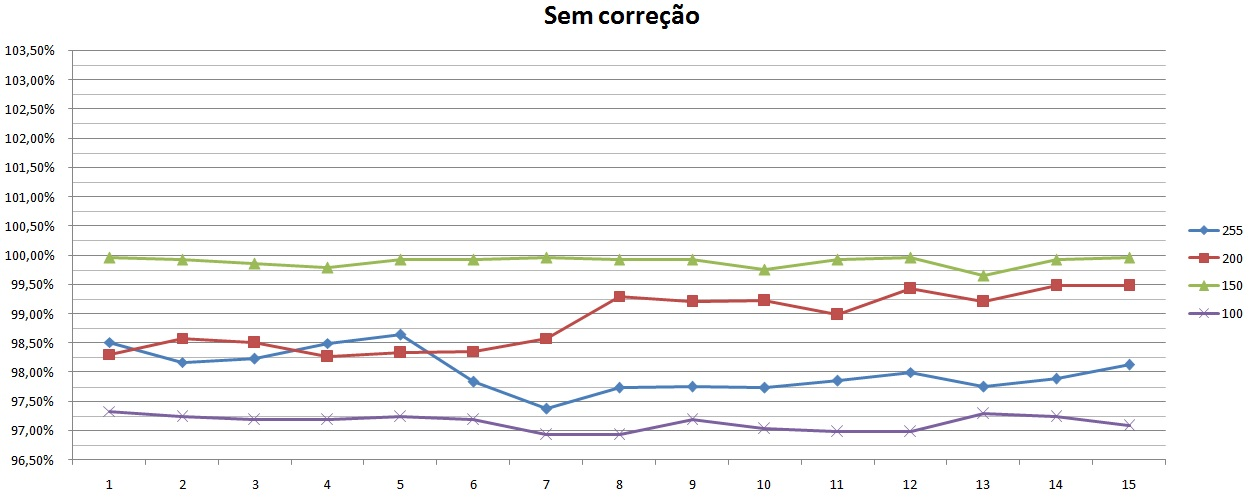
\includegraphics[width=1\textwidth]{semcorrecao.jpg}
	\caption{Velocidades do motor A em relação ao motor B em \%, quinze comparações para cada valor de PWM. Valores de PWM testados: 100, 150, 200 e 255}
	\label{fig:semcorrecao}
\end{figure}

Como podemos ver no gráfico acima, todos os valores mesmo os mais próximos a 100\% estão abaixo de 100\%, ou seja, em todos os testes e nas quatro potencias (PWMs) testadas o motor A permanece com uma velocidade inferior a velocidade do motor B, comprovando a necessidade de controle e também prova a diferença entre os motores mesmo sendo ``iguais". Também podemos observar que as diferenças no PWM se mostram maiores.

Com os resultados acima \ref{fig:semcorrecao} apresentados foi proposto dois métodos para o calculo dos pesos. O primeiro \ref{calib100} utilizando apenas o PWM mais discrepante na obtenção de amostas\ref{getamostras}, neste trabalho o PWM 100, o segundo método \ref{calibmult} é a utilização dos quatro valores de PWM no momento das coletas de amostras \ref{getamostras}.

\subsection{Pesos com PWM 100} \label{calib100}
Para calcular os pesos utilizando apenas como referencia o PWM 100, foi utilizado a função \textbf{getAmostras(100)} quatro vezes, tendo como resultado a seguinte tabela \ref{Tab:calib100}.
\begin{table}[!h]
	\renewcommand{\arraystretch}{1.3}
	\centering
	\begin{tabular}{|c|cc|}
		\hline
		Amostra \# & Motor A & Motor B \\ \hline
		    1      & 127.87  & 131.93  \\
		    2      & 128.73  & 132.27  \\
		    3      & 128.80  & 132.53  \\
		    4      & 129.07  & 132.60  \\ \hline
	\end{tabular}
	\caption[Tabela de amotas PWM 100]{Tabela com a média de quatro amostras coletadas utilizando a função \textbf{getAmostras(100)}.}
	\label{Tab:calib100}
\end{table}
Lembrando que a função \textbf{getAmostras(int \_PWM)} \ref{getamostras} utiliza a função \textbf{processMedia()} \ref{processmedia} ao fim de cada execução, ou seja, a função geradora de média é executada quatro vezes gerando os as médias acima \ref{Tab:calib100} apresentadas.
Ao fim das coletas passamos para o passo ao qual efetivamente calcula-se os pesos utilizando-se da função \textbf{finalMedia()} \ref{finalMedia}, como explicado a função determina o somando-se as médias de velocidade obtidas do motor A dividindo-a pelo numero de amostras(quatro), somando-se as médias de velocidade do motor B e também dividindo pelo numero de amostras, tendo as duas médias do somatório da média é realizado uma proporção com uma regra de três básica, assumindo o menor valor como o valor máximo(100\%), então obtemos os pesos, conforme os dados do estudo o peso do motor A, representado pela variável \textbf{pesoA} o valor de 1 (100\%) e a variável \textbf{pesoB} representando o valor do peso do motor B com o valor de 0.97 (97\%).
\begin{lstlisting}
void motorRefresh() {
	PWM_valA *= pesoA;
	PWM_valB *= pesoB;
	PWM_valA = int(PWM_valA);
	PWM_valB = int(PWM_valB);
	analogWrite(PWMA, PWM_valA);
	analogWrite(PWMB, PWM_valB);
}
\end{lstlisting}
Com os pesos determinados sempre o programa fizer uma alteração nos valores de PWM dos motores, utilizando a função \textbf{motorRefresh()} acima descrita, este será multiplicado pelo seu respectivo peso antes de alterar efetivamente a velocidade. Sendo assim o robô calibrado com as configurações de peso acima, ao selecionar o PWM de valor 100 para ambos os motores o valor determinado para o motor A será de 100 porem o valor do motor B será de 97.

\subsubsection{Resultados calibragem de unico PWM}
Ao utilizar a calibragem acima citada, a qual utiliza apenas o PWM de valor 100 na tomada de amostras para calculo dos pesos, teve-se o seguinte resultado para os quatro PWMs (100, 150, 200 e 255).
\begin{figure}[H]	
	\centering
	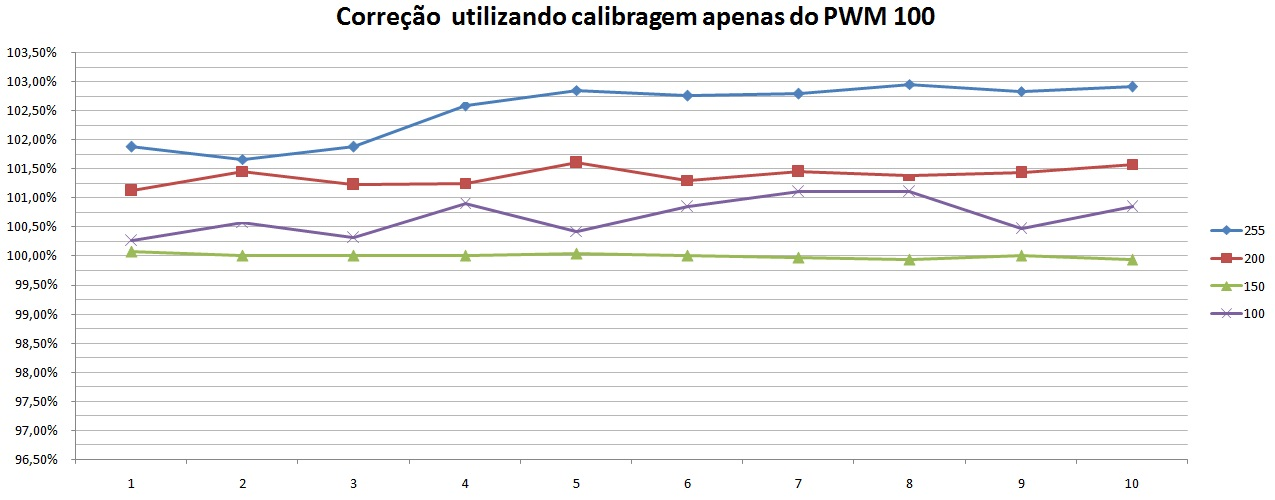
\includegraphics[width=1\textwidth]{correcao100.jpg}
	\caption{Velocidades do motor A em relação ao motor B em \%, quinze comparações para cada valor de PWM. Valores de PWM testados: 100, 150, 200 e 255}
	\label{fig:correcao100}
\end{figure}
No gráfico acima \ref{fig:correcao100} podemos ver claramente que o motor A passou a ser sempre mais rápido que o moto B, apenas mundo o erro de lado, o PWM de valor 150 passa a ser o mais preciso.

\subsection{Pesos com quatro PWMs} \label{calibmult}
Afim de aumentar a precisão das correções, foi utilizado quatro valores de PWM na fase de coleta de amostas \ref{getamostras}, tendo como resultado a seguinte tabela \ref{Tab:calibMC}.
\begin{table}[!h]
	\renewcommand{\arraystretch}{1.3}
	\centering
	\begin{tabular}{|c|c|cc|}
		\hline
		Amostra \# & PWM & Motor A & Motor B \\ \hline
		    1      & 255 & 347.40  & 355.33  \\
		    2      & 200 & 270.13  & 274.67  \\
		    3      & 150 & 198.87  & 202.80  \\
		    4      & 100 & 129.73  & 133.00  \\ \hline
	\end{tabular}
	\caption[Tabela de amotas PWM 100]{Tabela com a média de quatro amostras coletadas utilizando a função \textbf{getAmostras(100); getAmostras(150); getAmostras(200); getAmostras(255)}.}
	\label{Tab:calibMC}
\end{table}
Ao fim da coleta de amostras utilizando os quatro valores de PWM citados e ao fim da execução da função \textbf{finalMedia()} \ref{finalMedia} temos os valores de 1(100\%) para o \textbf{pesoA} e o valor de 0.98(98\%) para o \textbf{pesoB}. Assim como citado na sessão anterior os valores de PWM solicitados ao robô é multiplicado pelo seu peso antes de ser aplicado.

\subsubsection{Resultado calibragem com quatro valores PWMs}
Utilizando-se da configuração acima citada a qual foi utilizado as quatro amostragens para o calculo do peso temos o seguinte resultado.
\begin{figure}[H]	
	\centering
	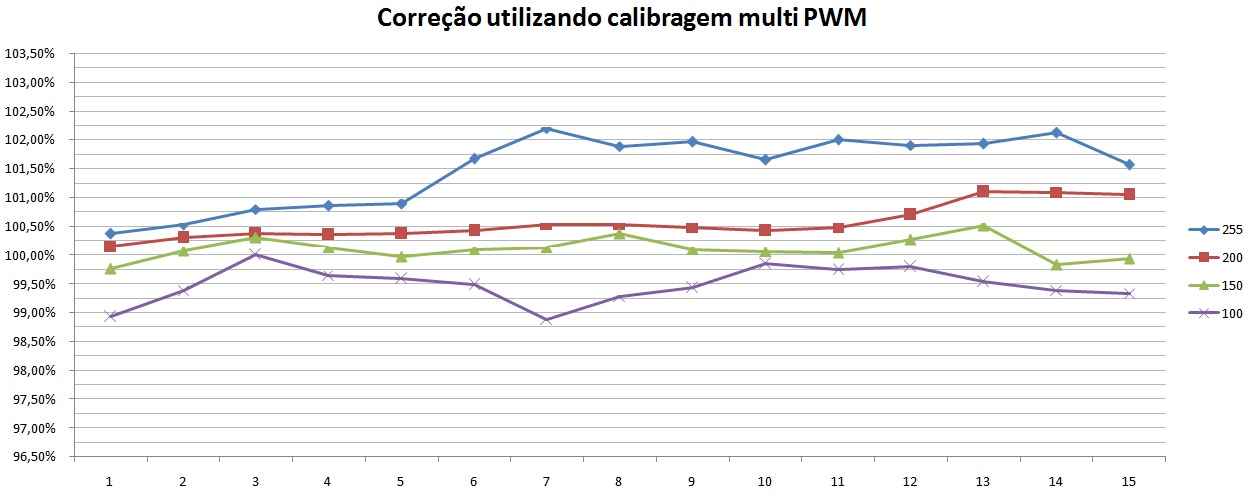
\includegraphics[width=1\textwidth]{correcao4pwm.jpg}
	\caption{Velocidades do motor A em relação ao motor B em \%, quinze comparações para cada valor de PWM. Valores de PWM testados: 100, 150, 200 e 255}
	\label{fig:correcao4pwm}
\end{figure}
Como podemos ver no gráfico acima o PWM 150 permanece mais estável que os demais valores tendo alguns testes abaixo de 100\% e outros acima. Notamos também que o robô se tornou mais equilibrado, tendo alguns valores de PWM com o motor A mais rápido e outros valores tendo o motor B como mais rápido, deixando assim o robô mais equilibrado.

\chapter{Conclusão}
Com base nos estudo realizados até o momento é fato que os motores necessitam de uma pequena correção para trabalharem de forma equivalente em relação as suas velocidades. Podemos também concluir pela analise do gráfico \ref{fig:semcorrecao} que cada regime de potencia requer uma correção diferente e também que os regimes de grande potencia (PWMs acima dos 200, sabe-se que o maior valor é 255) se mostram menos estáveis. Analisemos então os quatro regimes de potencia (PWMs) separadamente, começando com o PWM de valor 100.

Nos gráficos a seguir a linha azul \textbf{(Ñ Calib $\lozenge$)} refere-se aos valores obtidos nos testes \ref{fig:semcorrecao} sem calibragem, a linha vermelha \textbf{(Mono Calib $\Box$)} aos valores obtidos nos testes \ref{fig:correcao100} utilizando apenas o PWM 100 para calibragem e por ultimo a linha verde \textbf{(Multi Calib $\triangle$)} representando os valores nos testes \ref{fig:correcao4pwm} o qual foi utilizado quatro valores de PWM para a calibragem.

\section{Analise do PWM 100}\label{pwm100}
\begin{figure}[H]	
	\centering
	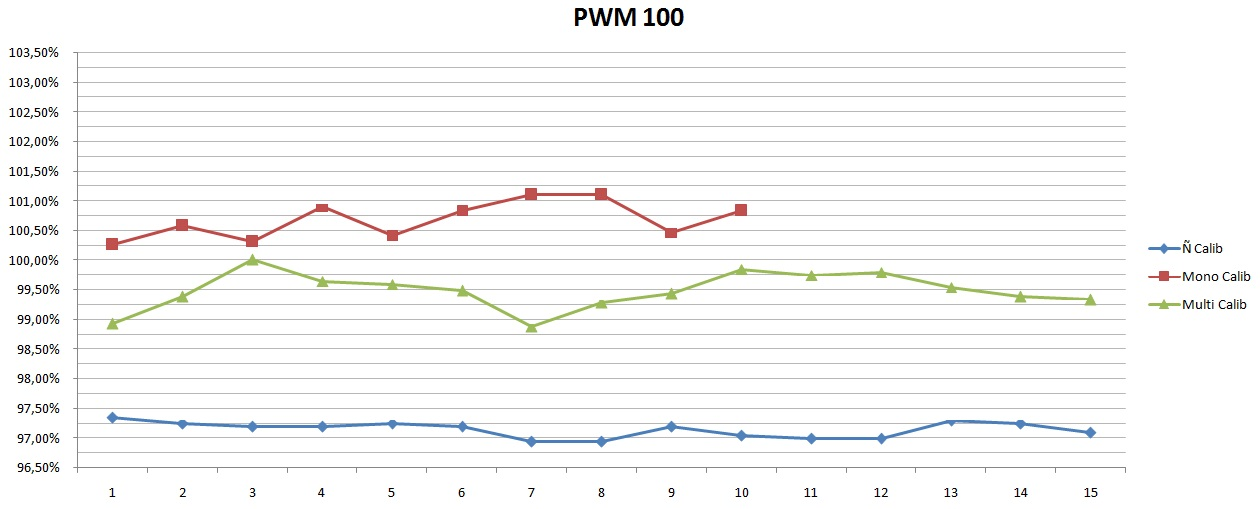
\includegraphics[width=1\textwidth]{pwm100.jpg}
	\caption{Velocidades do motor A em relação ao motor B em \%, quinze comparações para o valor de PWM 100.}
	\label{fig:pwm100}
\end{figure}
Com os dados deste gráfico podemos notar que o PWM 100 se mostra estável tendo em sua maior variação em apenas 1\% entre o teste 1 e 3, pode-se ver que as correções com um(linha vermelha) ou quatro valores de PWM(linha verde) na calibragem são eficientes, para equalização das velocidades dos motores tendo diferença de apenas 1\% para o motor A ou para o motor B, o qual sem correção (linha azul) apresentou um erro superior a 2\%.

\section{Analise do PWM 150}\label{pwm150}
\begin{figure}[H]	
	\centering
	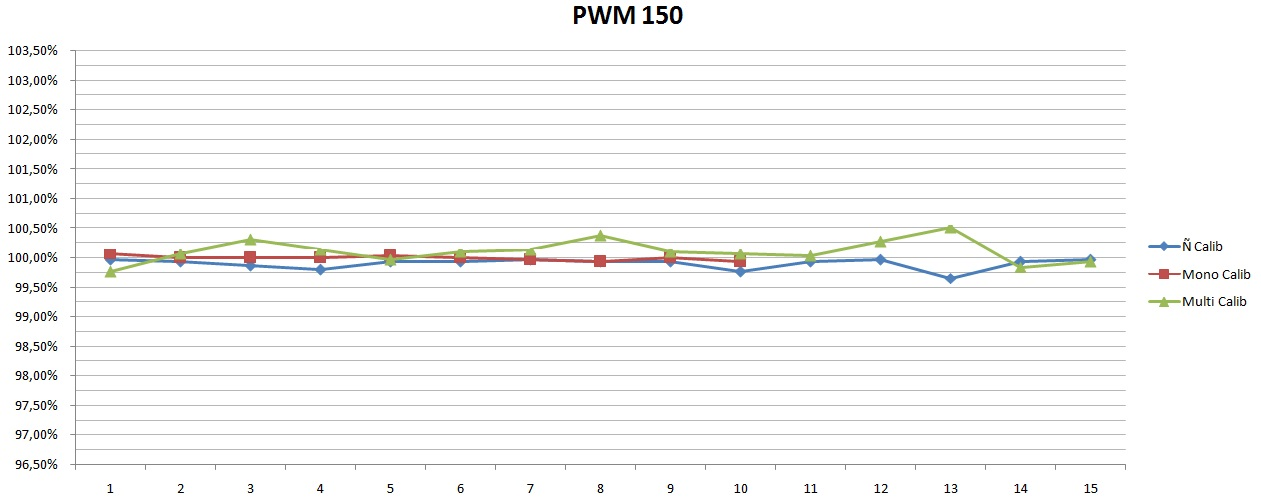
\includegraphics[width=1\textwidth]{pwm150.jpg}
	\caption{Velocidades do motor A em relação ao motor B em \%, quinze comparações para o valor de PWM 150.}
	\label{fig:pwm150}
\end{figure}
Analisando separadamente os regimes de potencia podemos notar que o valor de PWM 150 se mostra o a potencia mais estável quando comparado as velocidades, no gráfico \ref{fig:pwm150} podemos ver claramente que em nos três casos a diferença de velocidades dos motores não foi superior a 0,5\% para mais ou para menos, tornando a correção quase desnecessária para este valor de PWM ou valores próximos a ele.

\section{Analise do PWM 200}\label{pwm200}
\begin{figure}[H]	
	\centering
	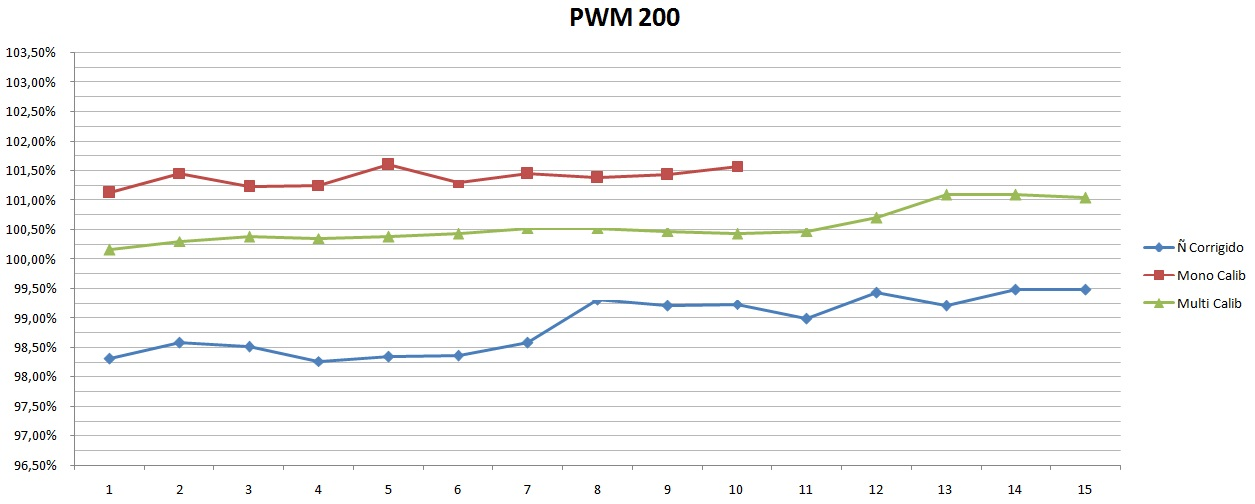
\includegraphics[width=1\textwidth]{pwm200.jpg}
	\caption{Velocidades do motor A em relação ao motor B em \%, quinze comparações para o valor de PWM 200.}
	\label{fig:pwm200}
\end{figure}
O gráfico acima \ref{fig:pwm200} o qual projeta os três testes realizados com o valor de 200 para o PWM (equivalente a aproximadamente 78,43\% de toda a potencia disponível) podemos notar a variação de 0,5\% ou mais entre os testes. A correção mais eficiente para este regime de potencia foi o de calibragem múltipla \ref{fig:correcao4pwm}.

\section{Analise do PWM 255}\label{pwm255}
\begin{figure}[H]	
	\centering
	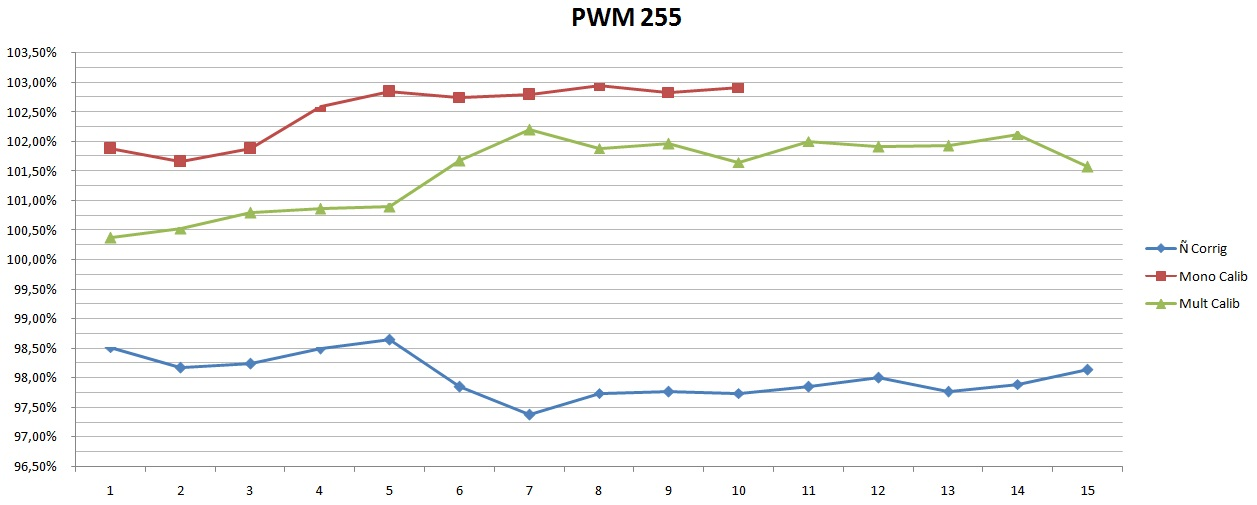
\includegraphics[width=1\textwidth]{pwm255.jpg}
	\caption{Velocidades do motor A em relação ao motor B em \%, quinze comparações para o valor de PWM 255.}
	\label{fig:pwm255}
\end{figure}
O regime de máxima potencia se demostrou o mais instável tendo variação superiores a 1\% entre os testes, acredita-se que por trata-se de máxima potencia os motores não mantém uma consistência em seu desempenho, deixando-o mais sensível a fatores externos ou variação da corrente disponível vinda das baterias, mesmo que a correção utilizando quatro valores de PWM \ref{fig:correcao4pwm} se mostrando mais eficiente em manter as velocidades parecidas, ainda sim demostra variações inesperadas. Tais variações -inconstâncias- podem ser notadas nas figuras \ref{fig:semcorrecao} e \ref{fig:correcao4pwm} com o PWM 255 (linhas azuis $\diamond$) e com o PWM de 200(linhas vermelhas $\Box$)\ref{pwm200}.



\chapter{Metodologia} \label{cap: metodologia}
Neste trabalho foi usado apenas um sensor para cada roda -os conectados aos pinos com interrupção\ref{isr}-, sendo os sensores mais externos da roda.
O funcionamento do encoder empregado neste trabalho é a de configuração mais simples apenas um sensor óptico, o qual realiza apenas a contagem de marcadores da fita que esta colada junto a roda conforme a figura \ref{fig:roda34marc}, convertendo o movimento angular das rodas em sinais digitais, estes sinais são utilizados como sinais de entrada para as interrupções \ref{isr}, realizando a contagem do numero de pulsos em determinado tempo.


\begin{enumerate}[(A)]
	
	\item Desenvolvimento e entrega do plano de trabalho;
	\item Escrita da introdução, levantamentos dos dados teóricos e bibliográficos.
	\item Revisão da literatura. 
	\item Implementar a aplicação
	\item Escritas do trabalho de conclusão do curso.		
	
	
\end{enumerate}

\chapter{Considerações Finais}


\vskip 10cm
\begin{table}[!h]
	\renewcommand{\arraystretch}{1.3}
	\centering
	\begin{tabular}{cccccccc}
		& & & & & & & \\
		Prof. Doc. Gedson Faria & & & & & & & Kelvim Rodrigues de Oliveira \\
		Orientador & & & & & & & Acadêmico \\
	\end{tabular}
\end{table}


\cleardoublepage
%\phantomsection
\addcontentsline{toc}{chapter}{Referências Bibliográficas} 
\bibliographystyle{abnt}
%\bibliographystyle{apalike} 
%\bibliographystyle{ieeetr} % Ordena por ordem de aparição.  
%\bibliographystyle{abbr} % Ordena por ordem alfabetica com nomes abreviados.
%\bibliographystyle{plain} % Ordena por ordem alfabetica com nomes por extenso.
\bibliography{bibliografia} % commented if *.bbl file included.

%\addcontentsline{toc}{chapter}{Ap\^endices}
%\appendix
%\include{apendice}

\end{document}